%% ------------------------------------------------------------------------- %%
\chapter{Moda das Ondas no Space Shooter para versão v3}
\label{sec:apend-moda-ss-v3}

Foram calculadas as modas das ondas do \textit{fitness} desenvolvido, para permitir a visualização dos inimigos mais comuns que o algoritmo convergiu.

%% ------------------------------------------------------------------------- %%
\section{Nave Parada com Disparo Amarelo}
\label{sec:apend-moda-ss-ys-v3}

\begin{figure}[H]
  \centering
  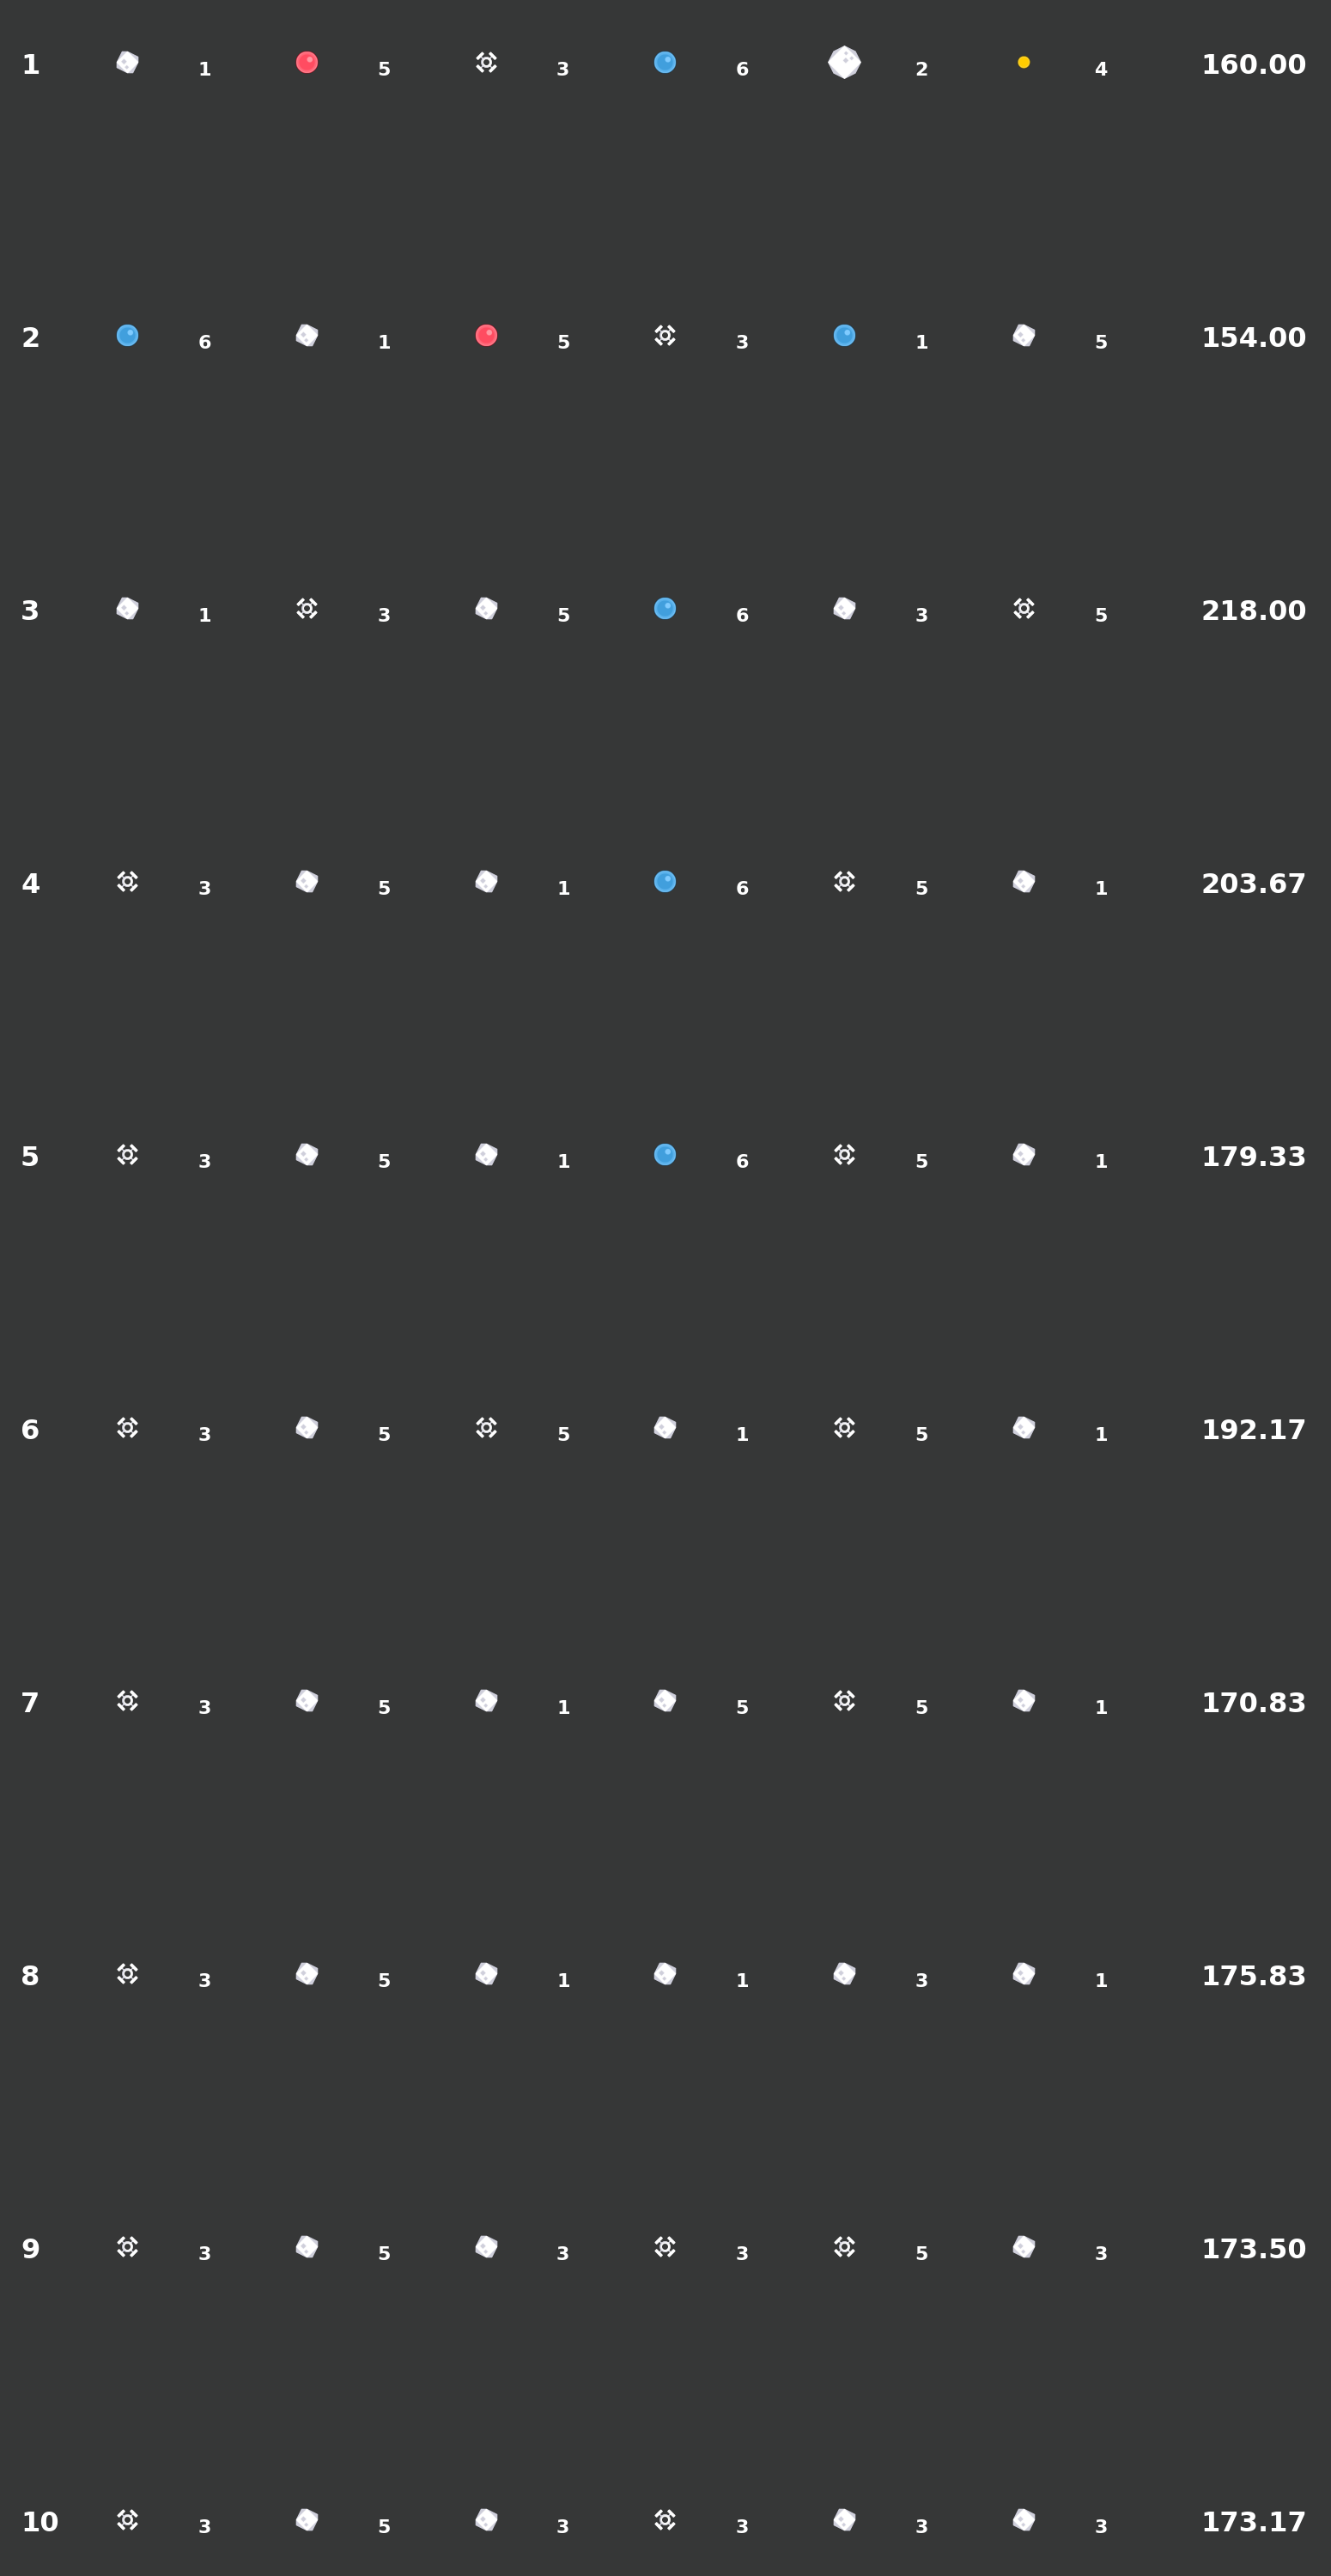
\includegraphics[width=0.7\textwidth]{figuras/ss/ss_yellowstill_ai_mode_2_1.png}
  \caption{Visualização da moda de cada onda com o fitness v3 contra Nave Parada, Disparo Amarelo.}
  \label{fig:ss-moda-ys-2-1}
\end{figure}

\begin{figure}[H]
  \centering
  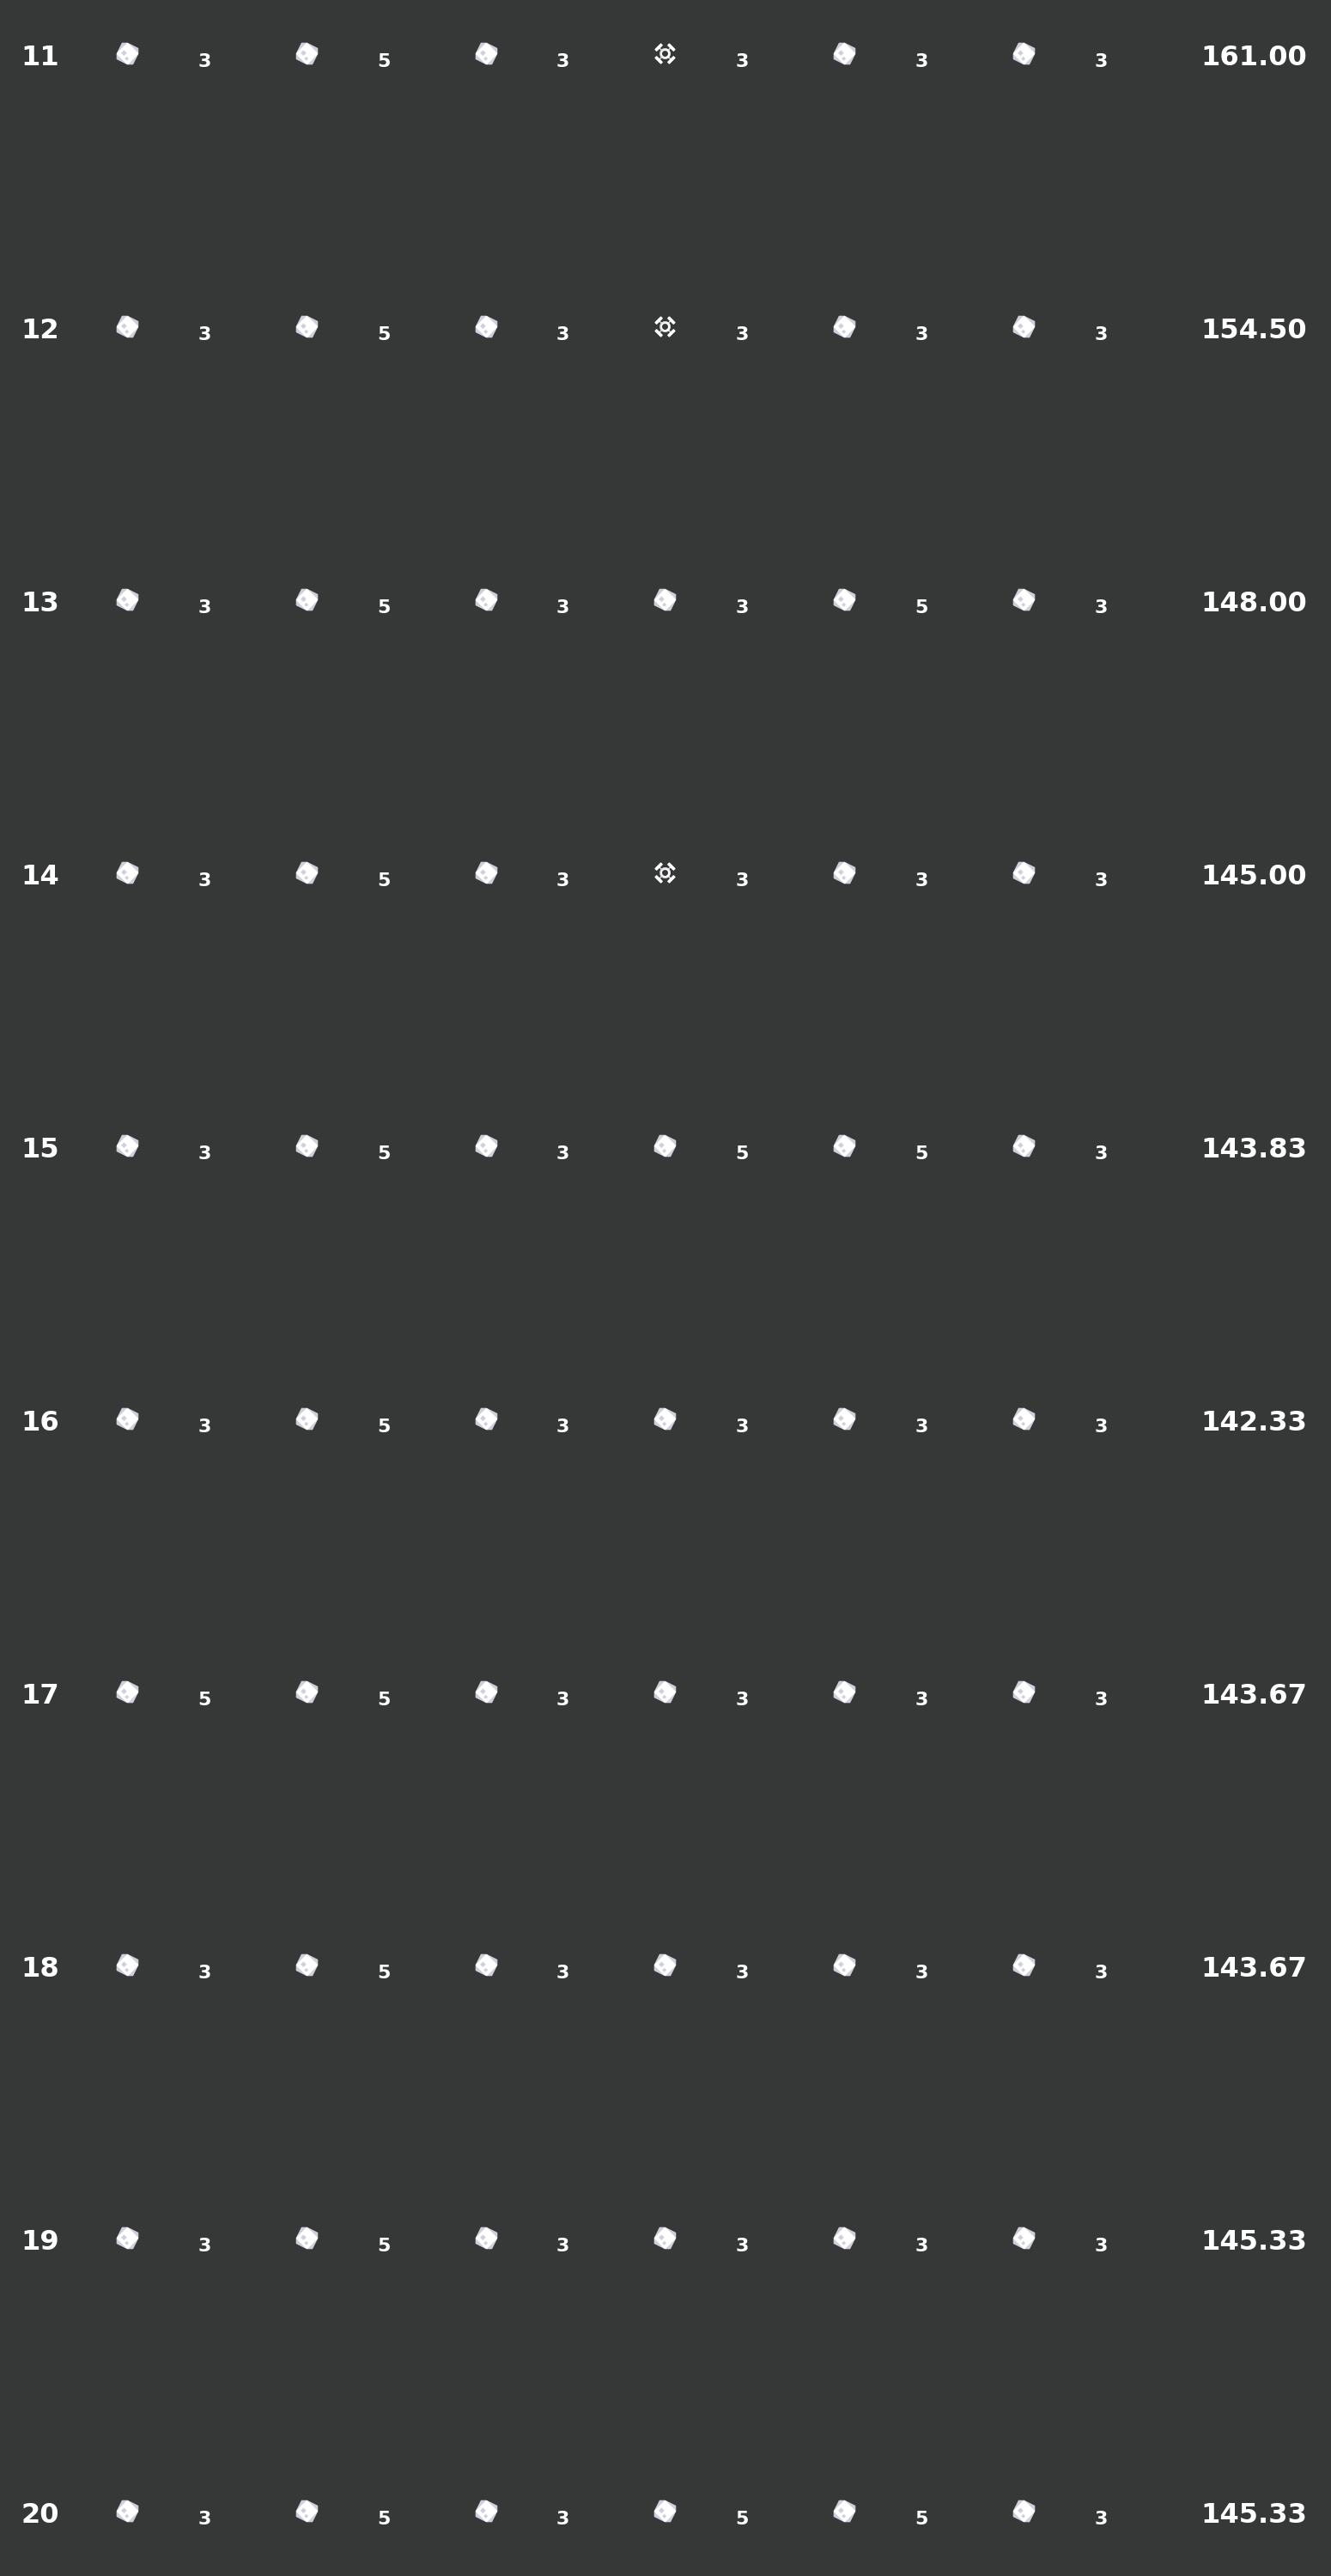
\includegraphics[width=0.7\textwidth]{figuras/ss/ss_yellowstill_ai_mode_2_2.png}
  \caption{Visualização da moda de cada onda com o fitness v3 contra Nave Parada, Disparo Amarelo.}
  \label{fig:ss-moda-ys-2-2}
\end{figure}

\begin{figure}[H]
  \centering
  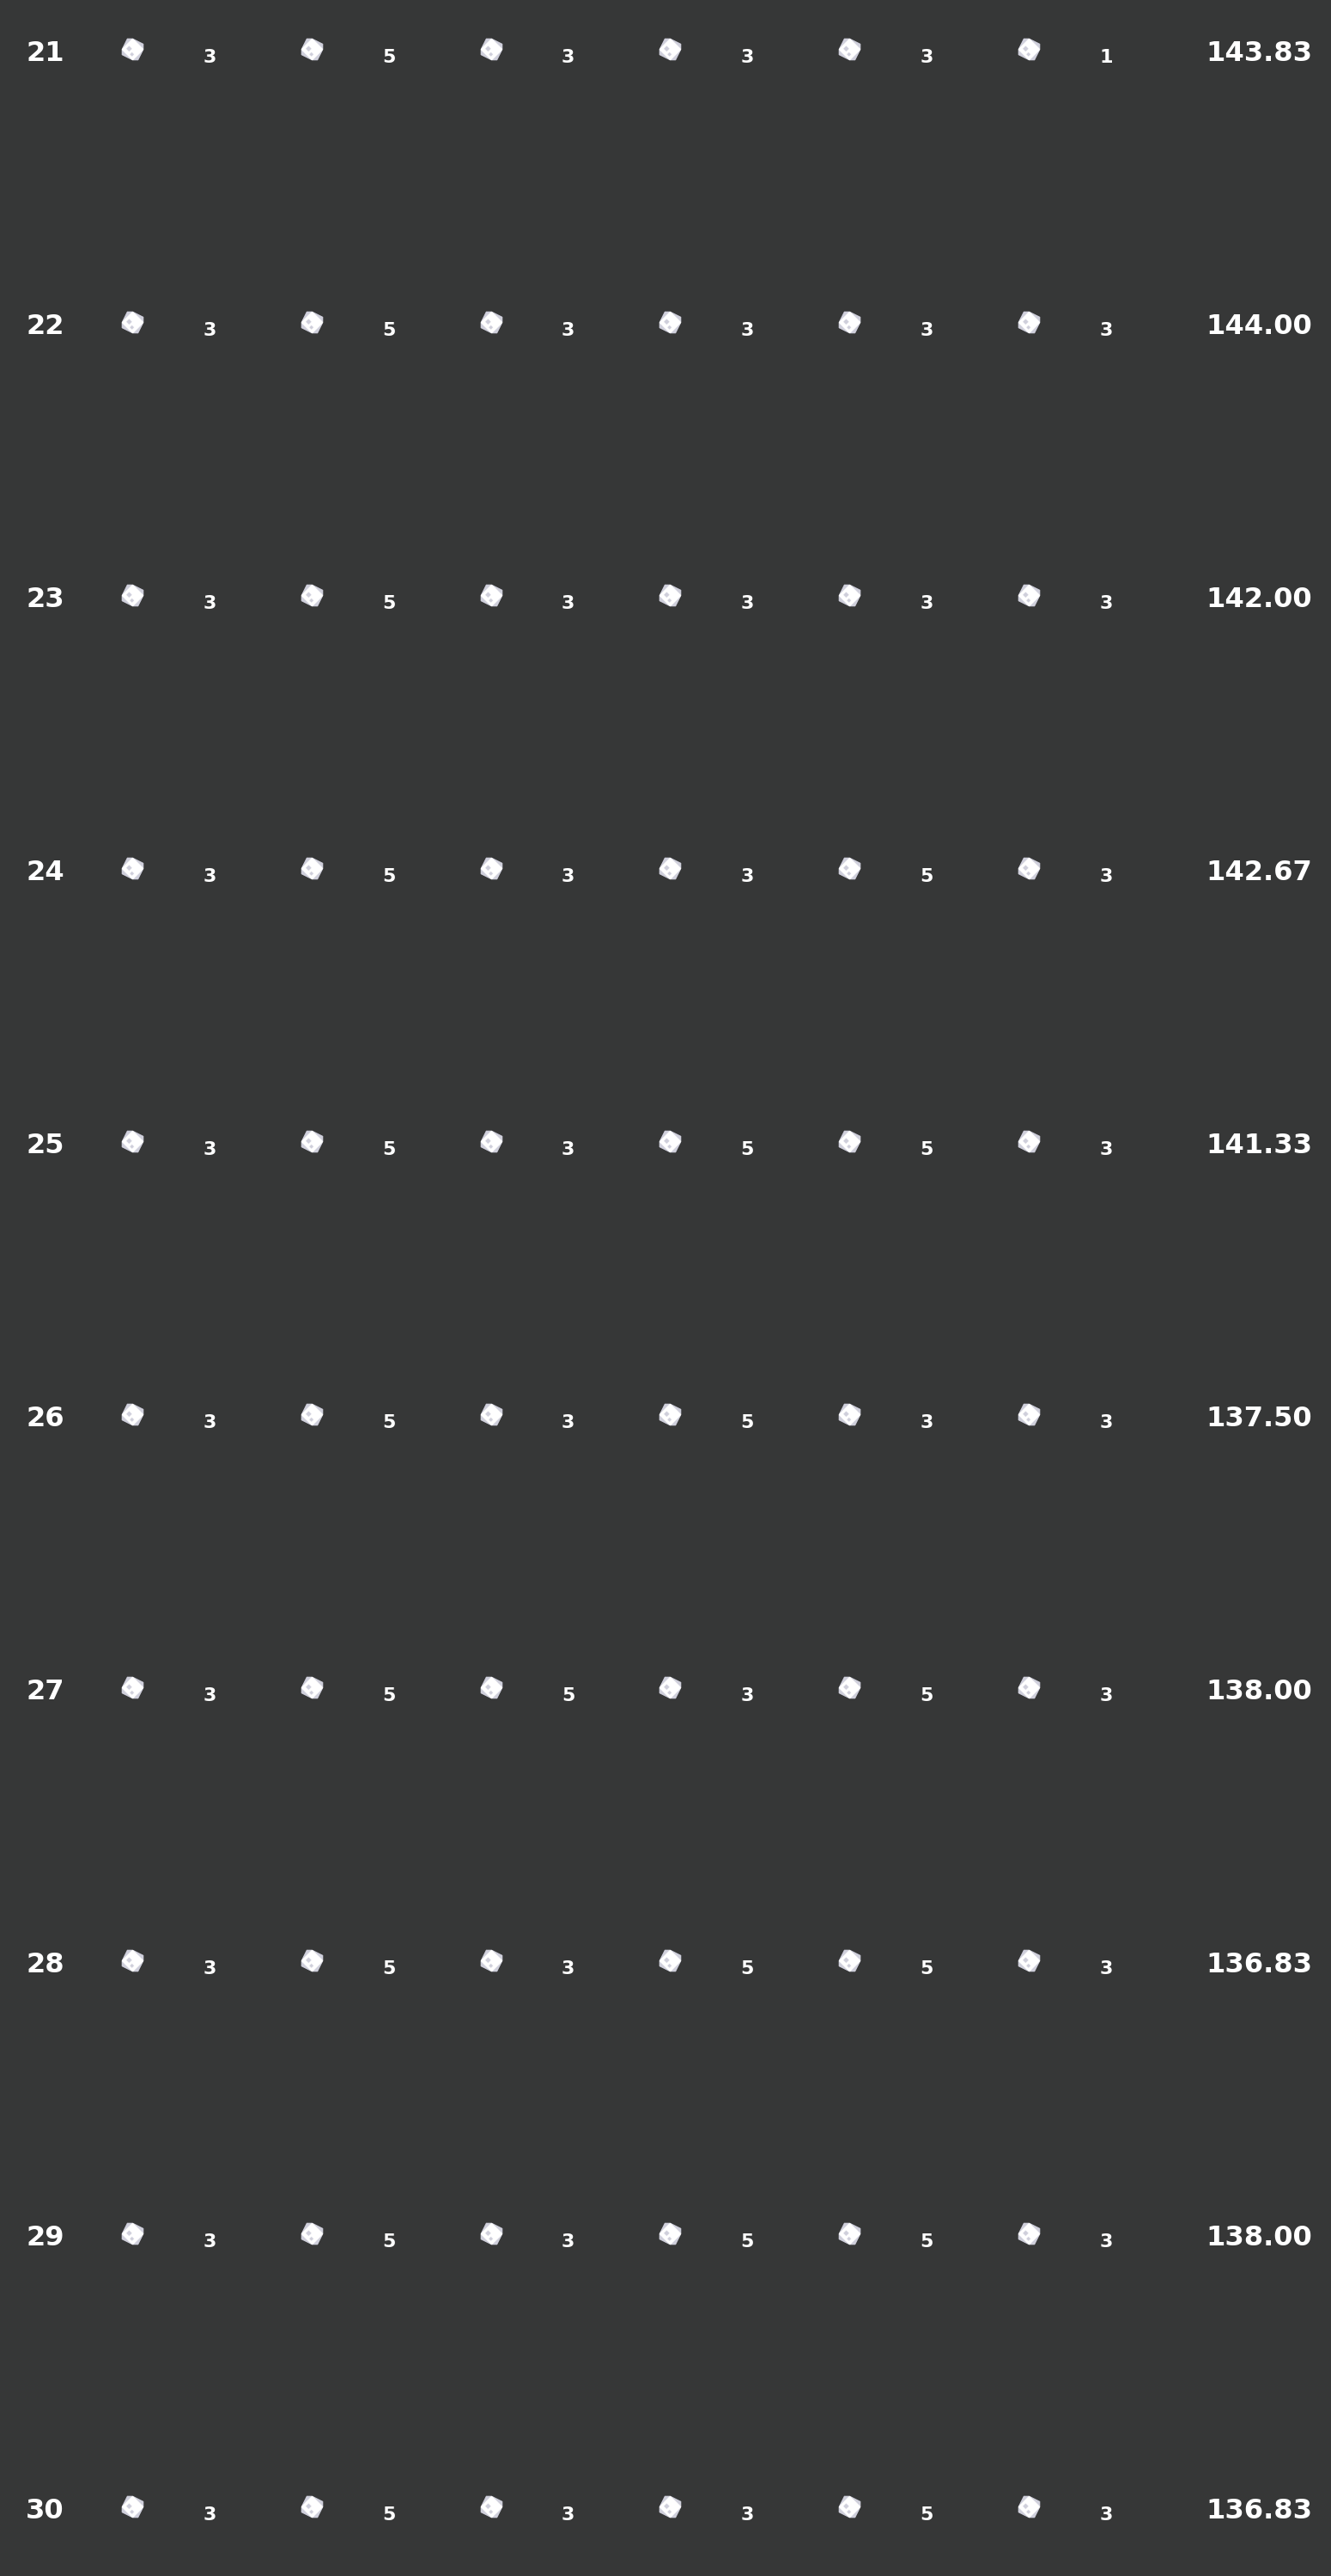
\includegraphics[width=0.7\textwidth]{figuras/ss/ss_yellowstill_ai_mode_2_3.png}
  \caption{Visualização da moda de cada onda com o fitness v3 contra Nave Parada, Disparo Amarelo.}
  \label{fig:ss-moda-ys-2-3}
\end{figure}

%% ------------------------------------------------------------------------- %%
\section{Nave Movendo com Disparo Amarelo}
\label{sec:apend-moda-ss-ym-v3}

\begin{figure}[H]
  \centering
  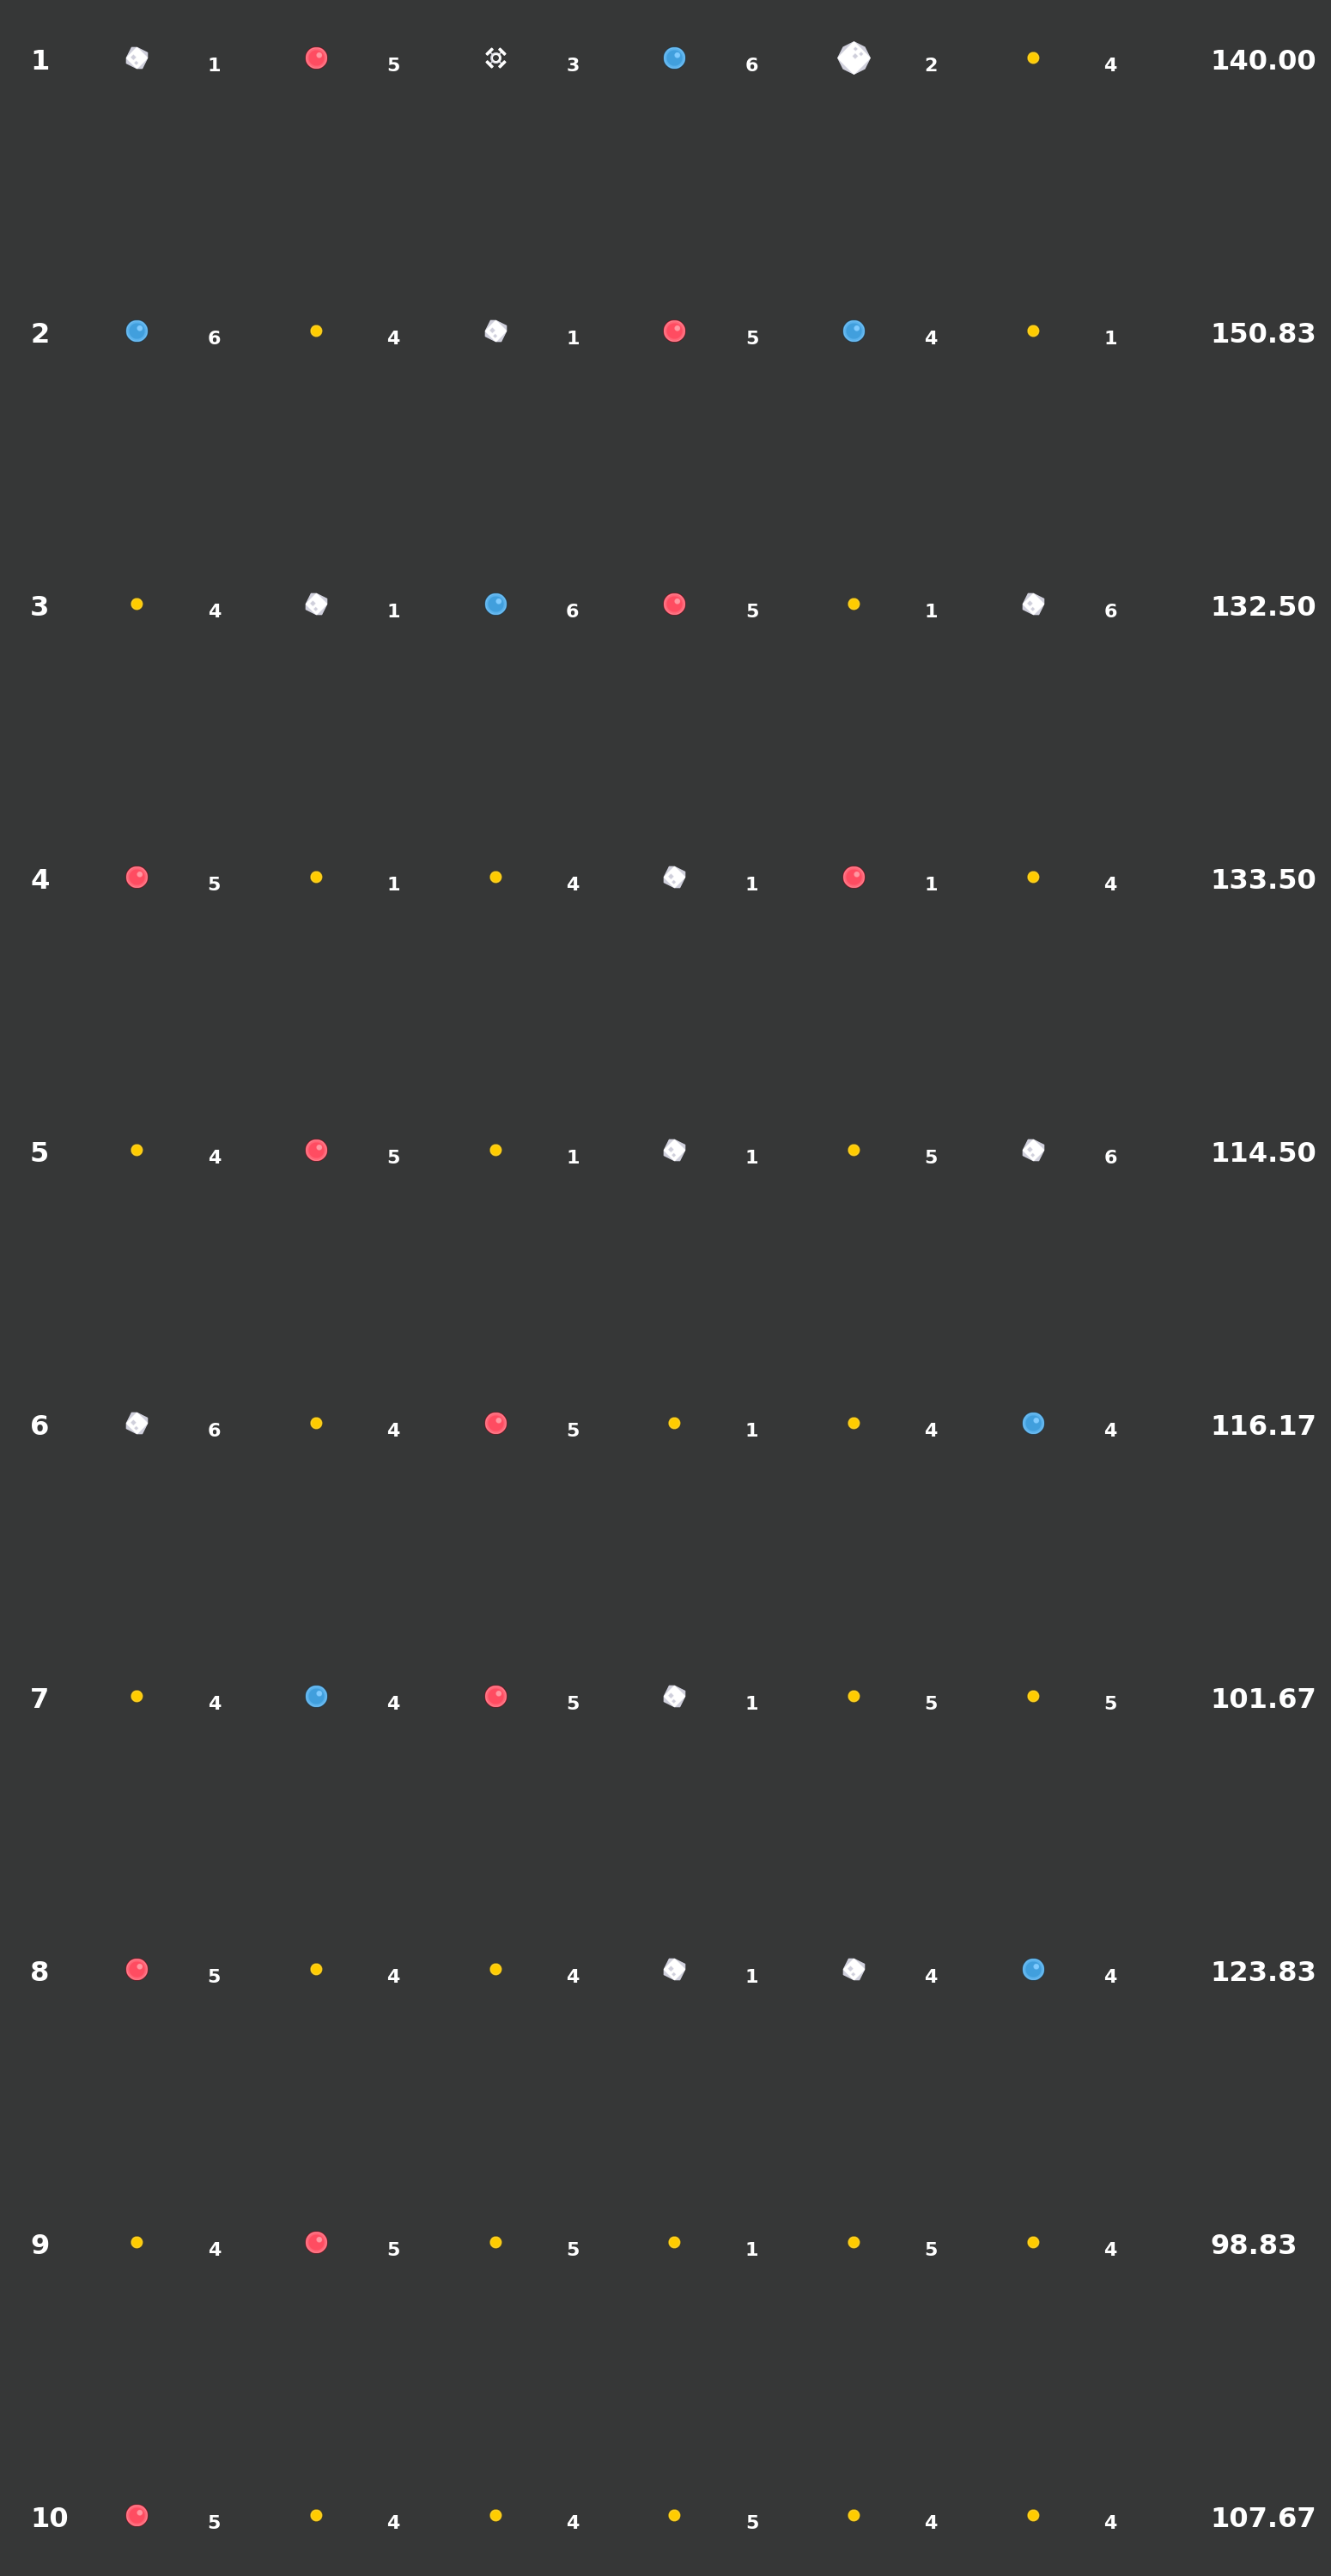
\includegraphics[width=0.7\textwidth]{figuras/ss/ss_yellowmove_ai_mode_2_1.png}
  \caption{Visualização da moda de cada onda com o fitness v3 contra Nave Movendo, Disparo Amarelo.}
  \label{fig:ss-moda-ym-2-1}
\end{figure}

\begin{figure}[H]
  \centering
  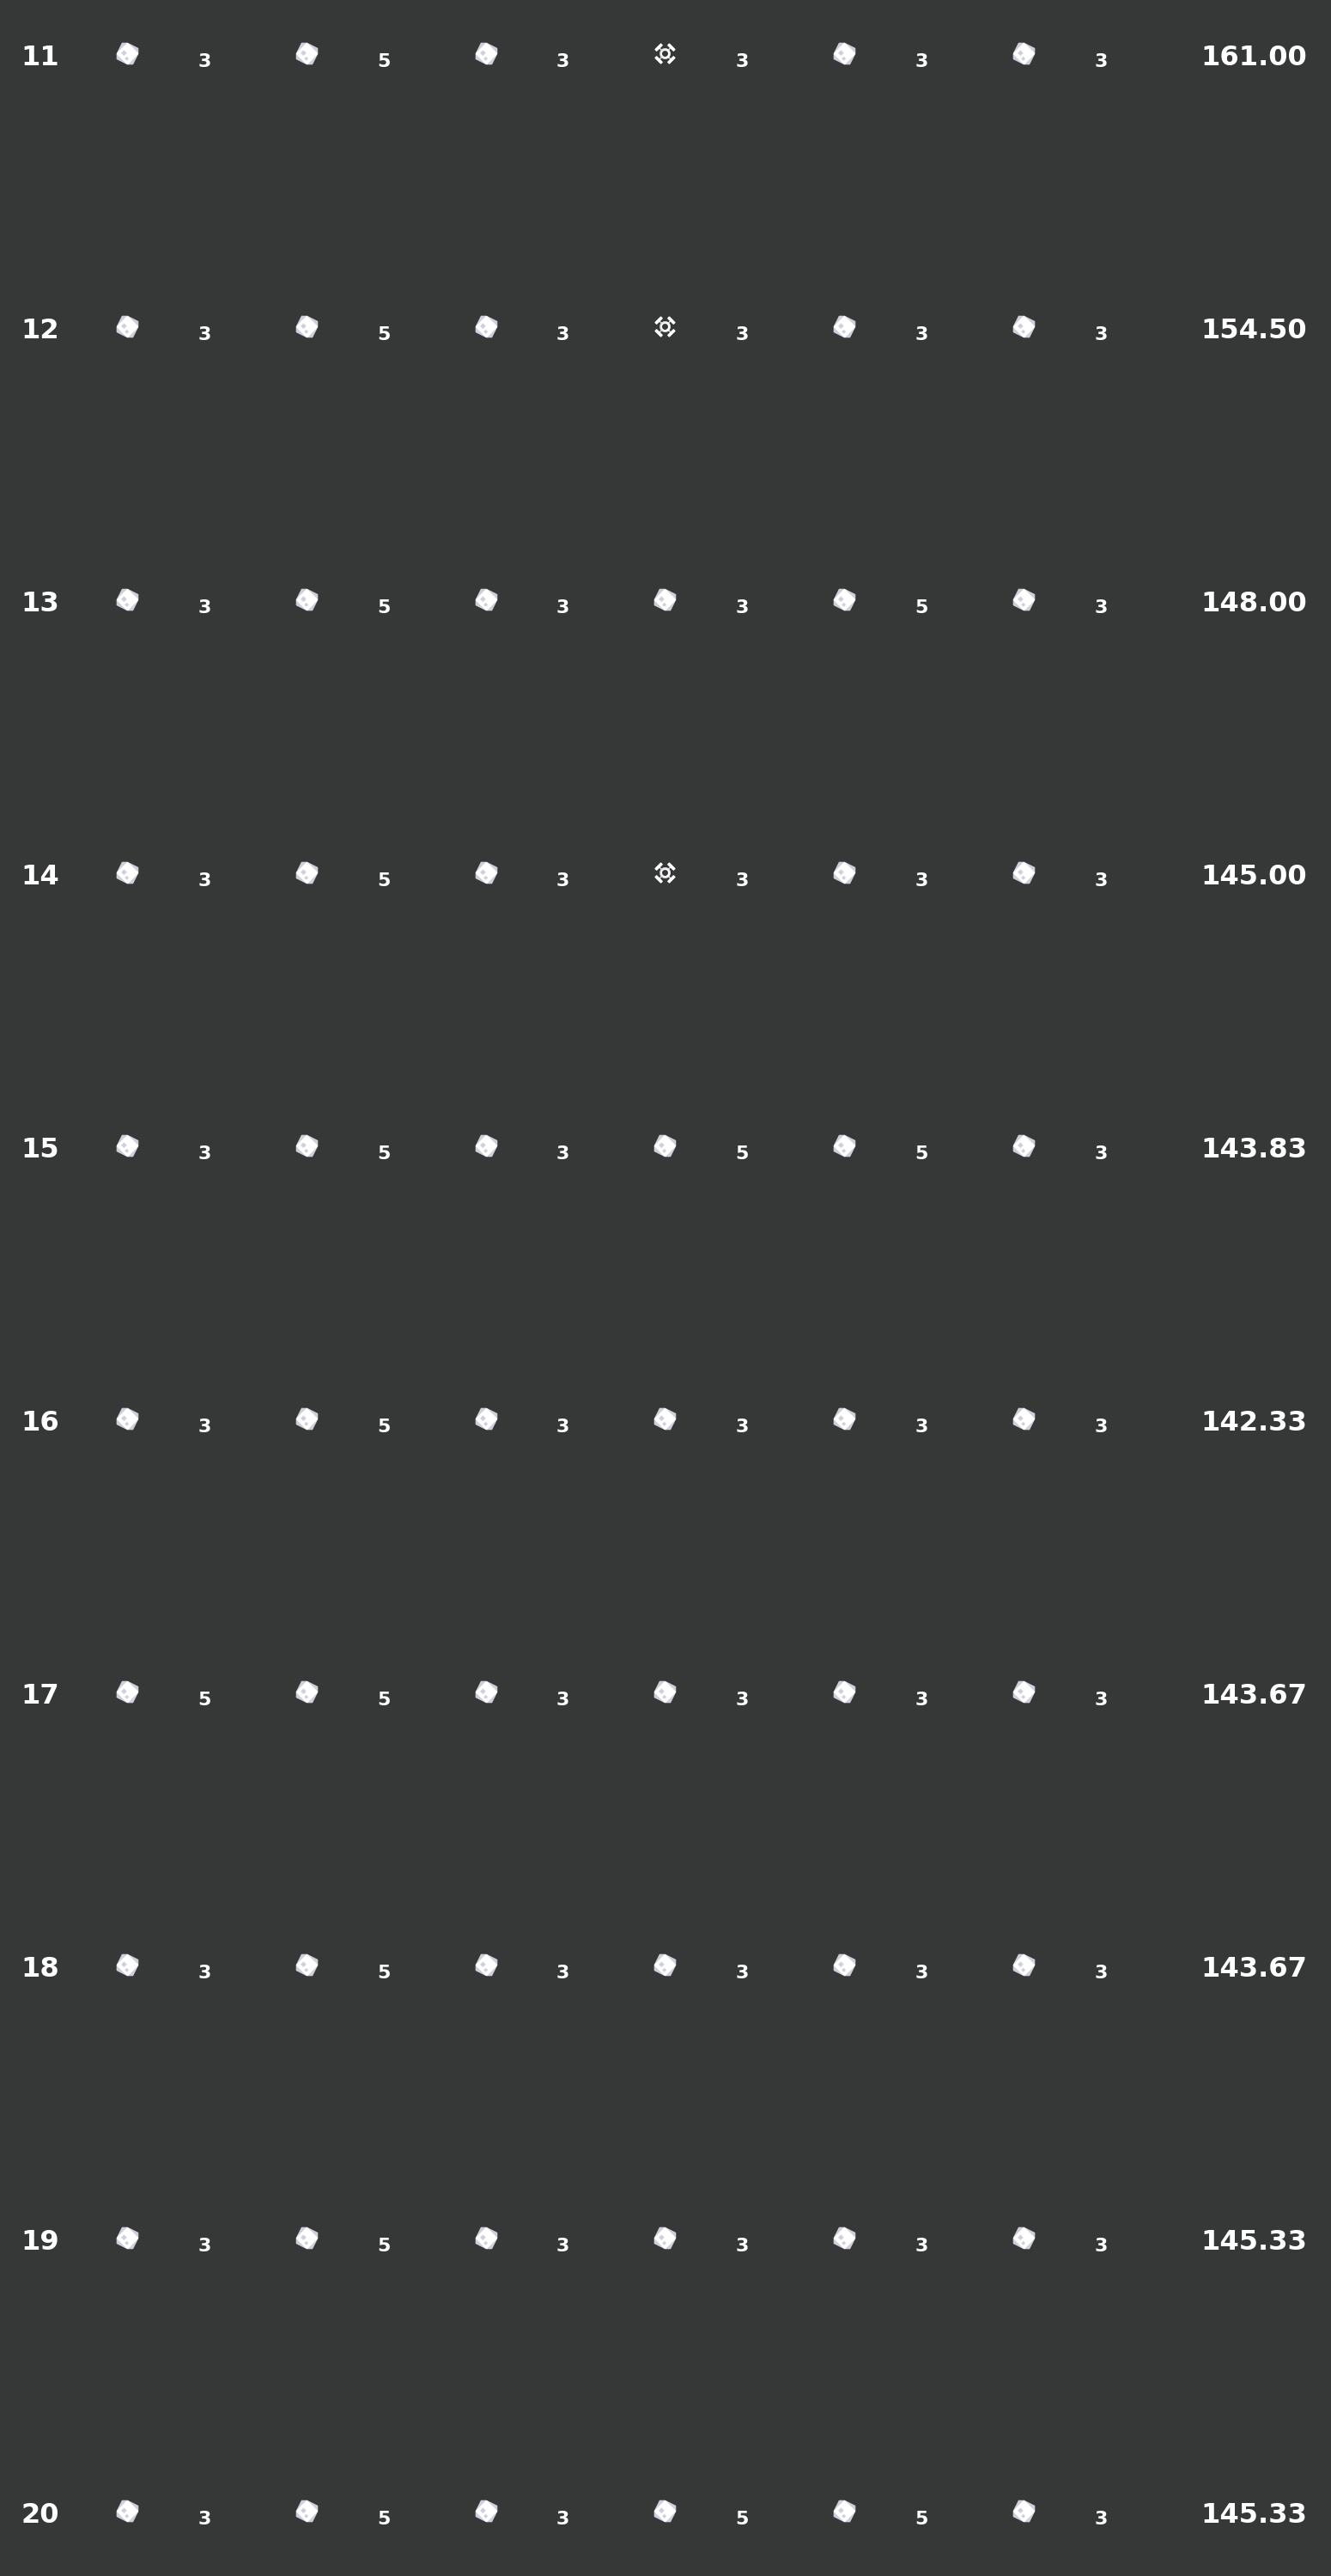
\includegraphics[width=0.7\textwidth]{figuras/ss/ss_yellowstill_ai_mode_2_2.png}
  \caption{Visualização da moda de cada onda com o fitness v3 contra Nave Movendo, Disparo Amarelo.}
  \label{fig:ss-moda-ym-2-2}
\end{figure}

\begin{figure}[H]
  \centering
  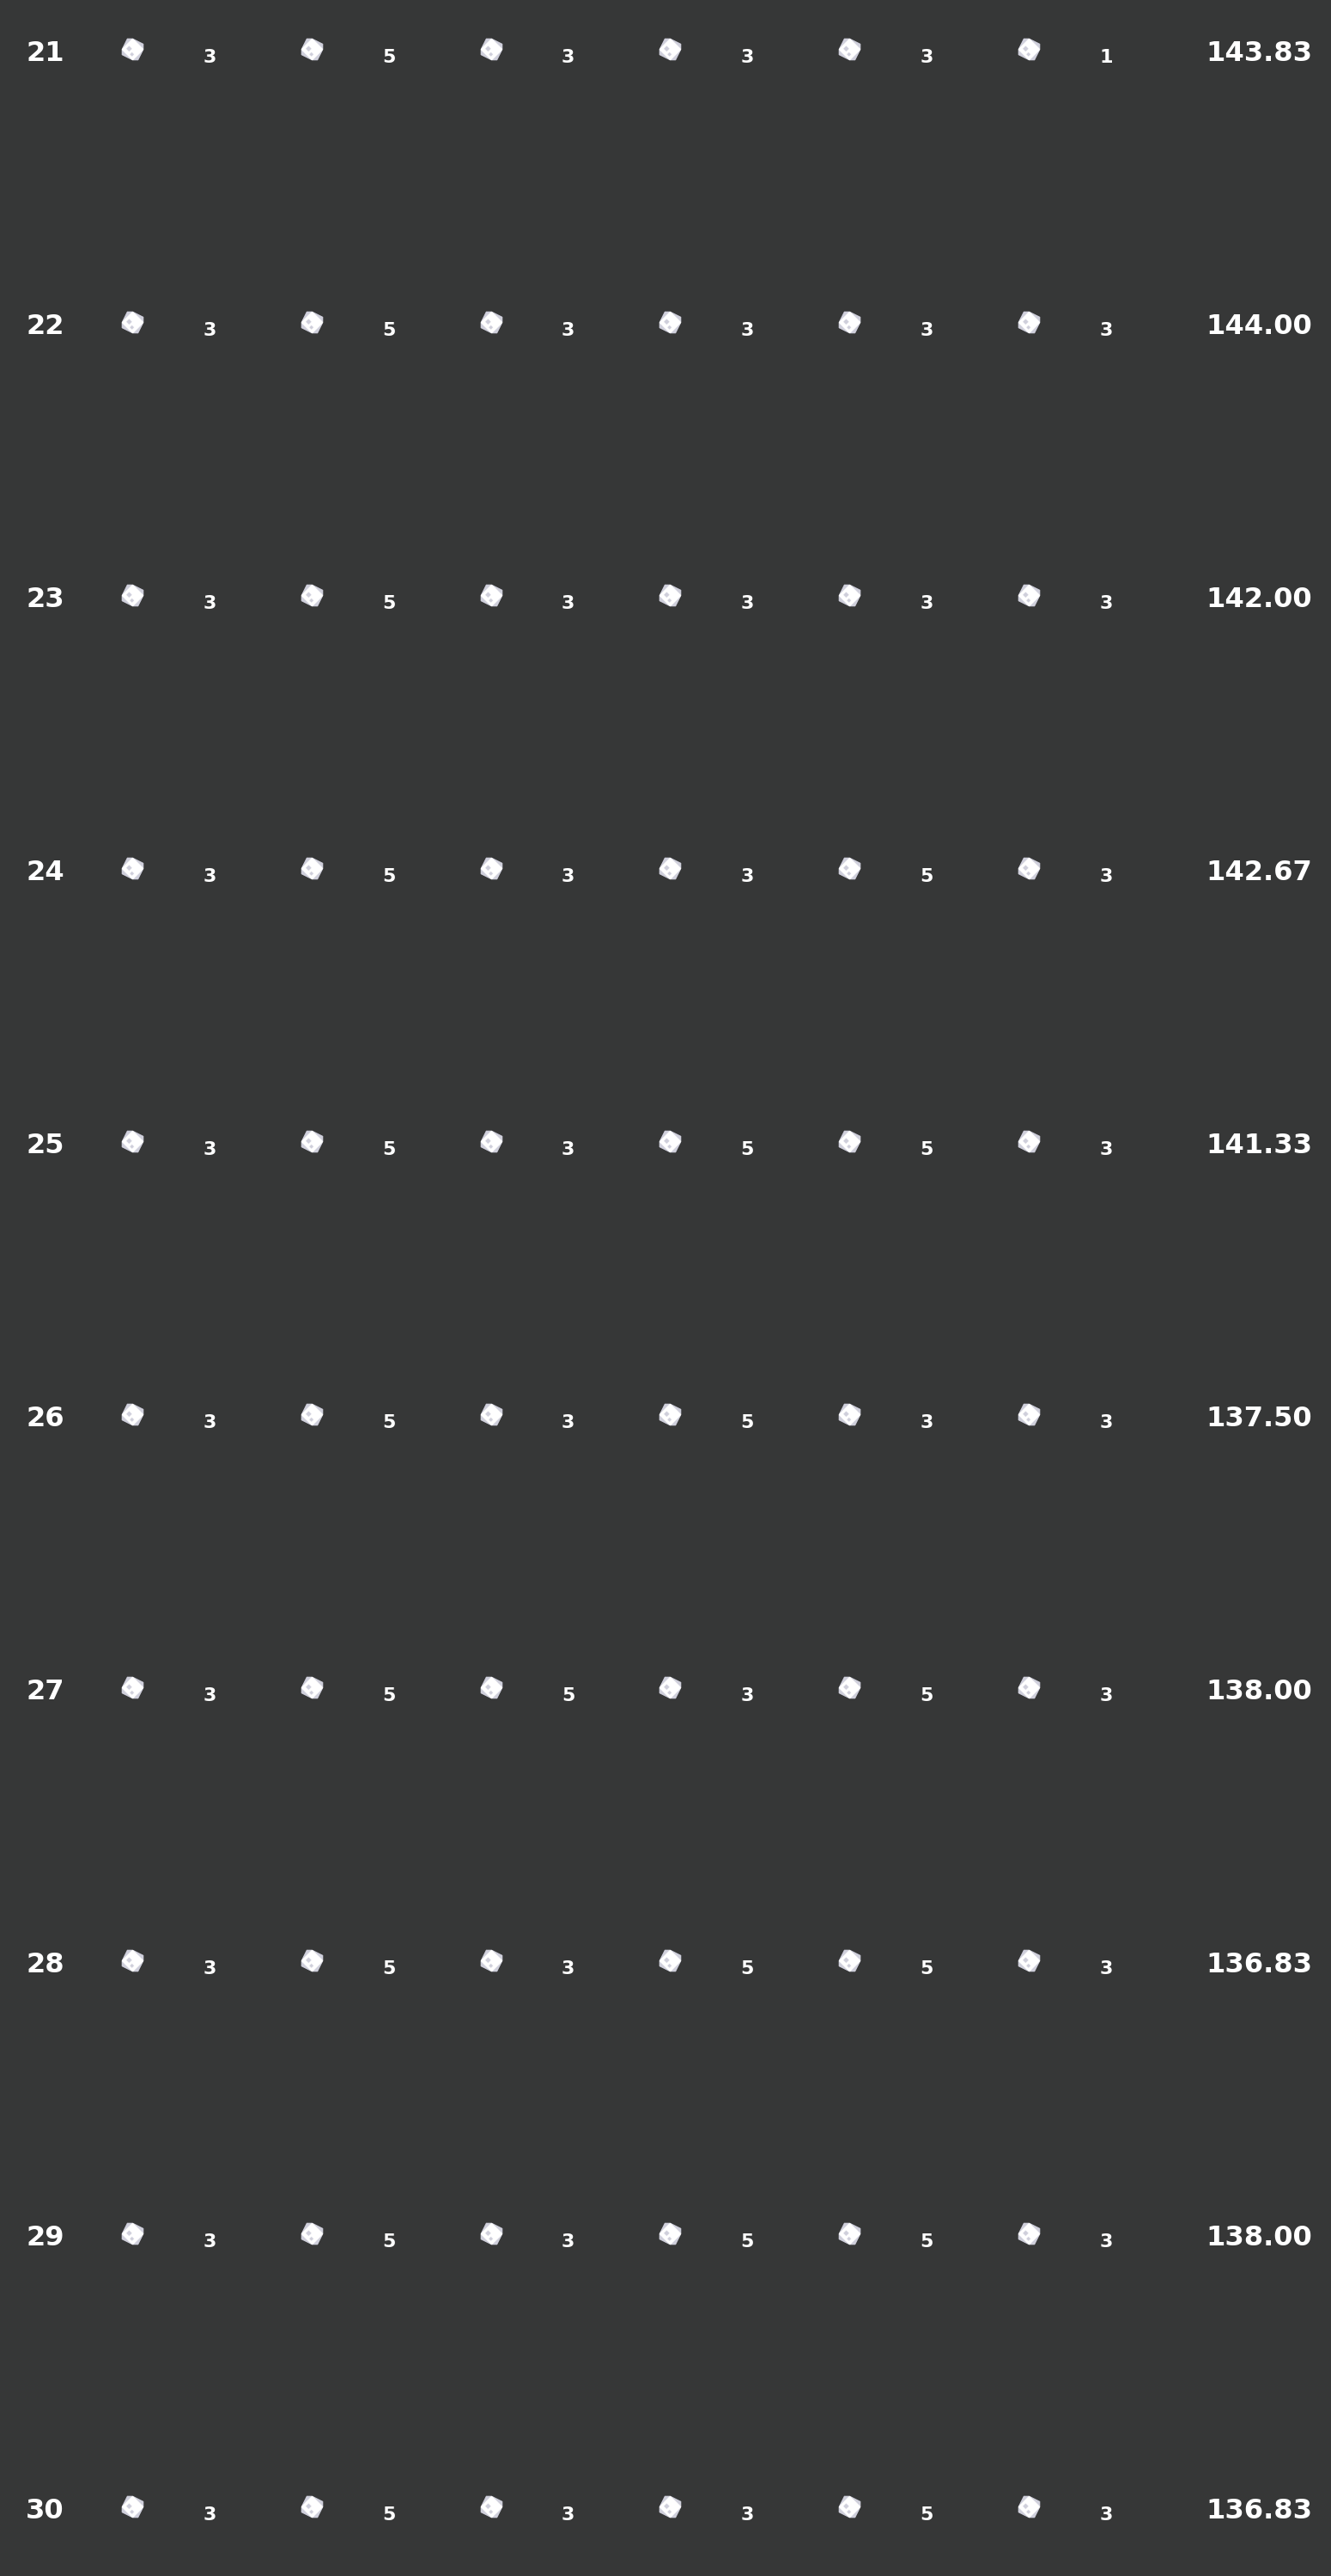
\includegraphics[width=0.7\textwidth]{figuras/ss/ss_yellowstill_ai_mode_2_3.png}
  \caption{Visualização da moda de cada onda com o fitness v3 contra Nave Movendo, Disparo Amarelo.}
  \label{fig:ss-moda-ym-2-3}
\end{figure}

%% ------------------------------------------------------------------------- %%
\section{Nave Parada com Disparo Vermelho}
\label{sec:apend-moda-ss-rs-v3}

\begin{figure}[H]
  \centering
  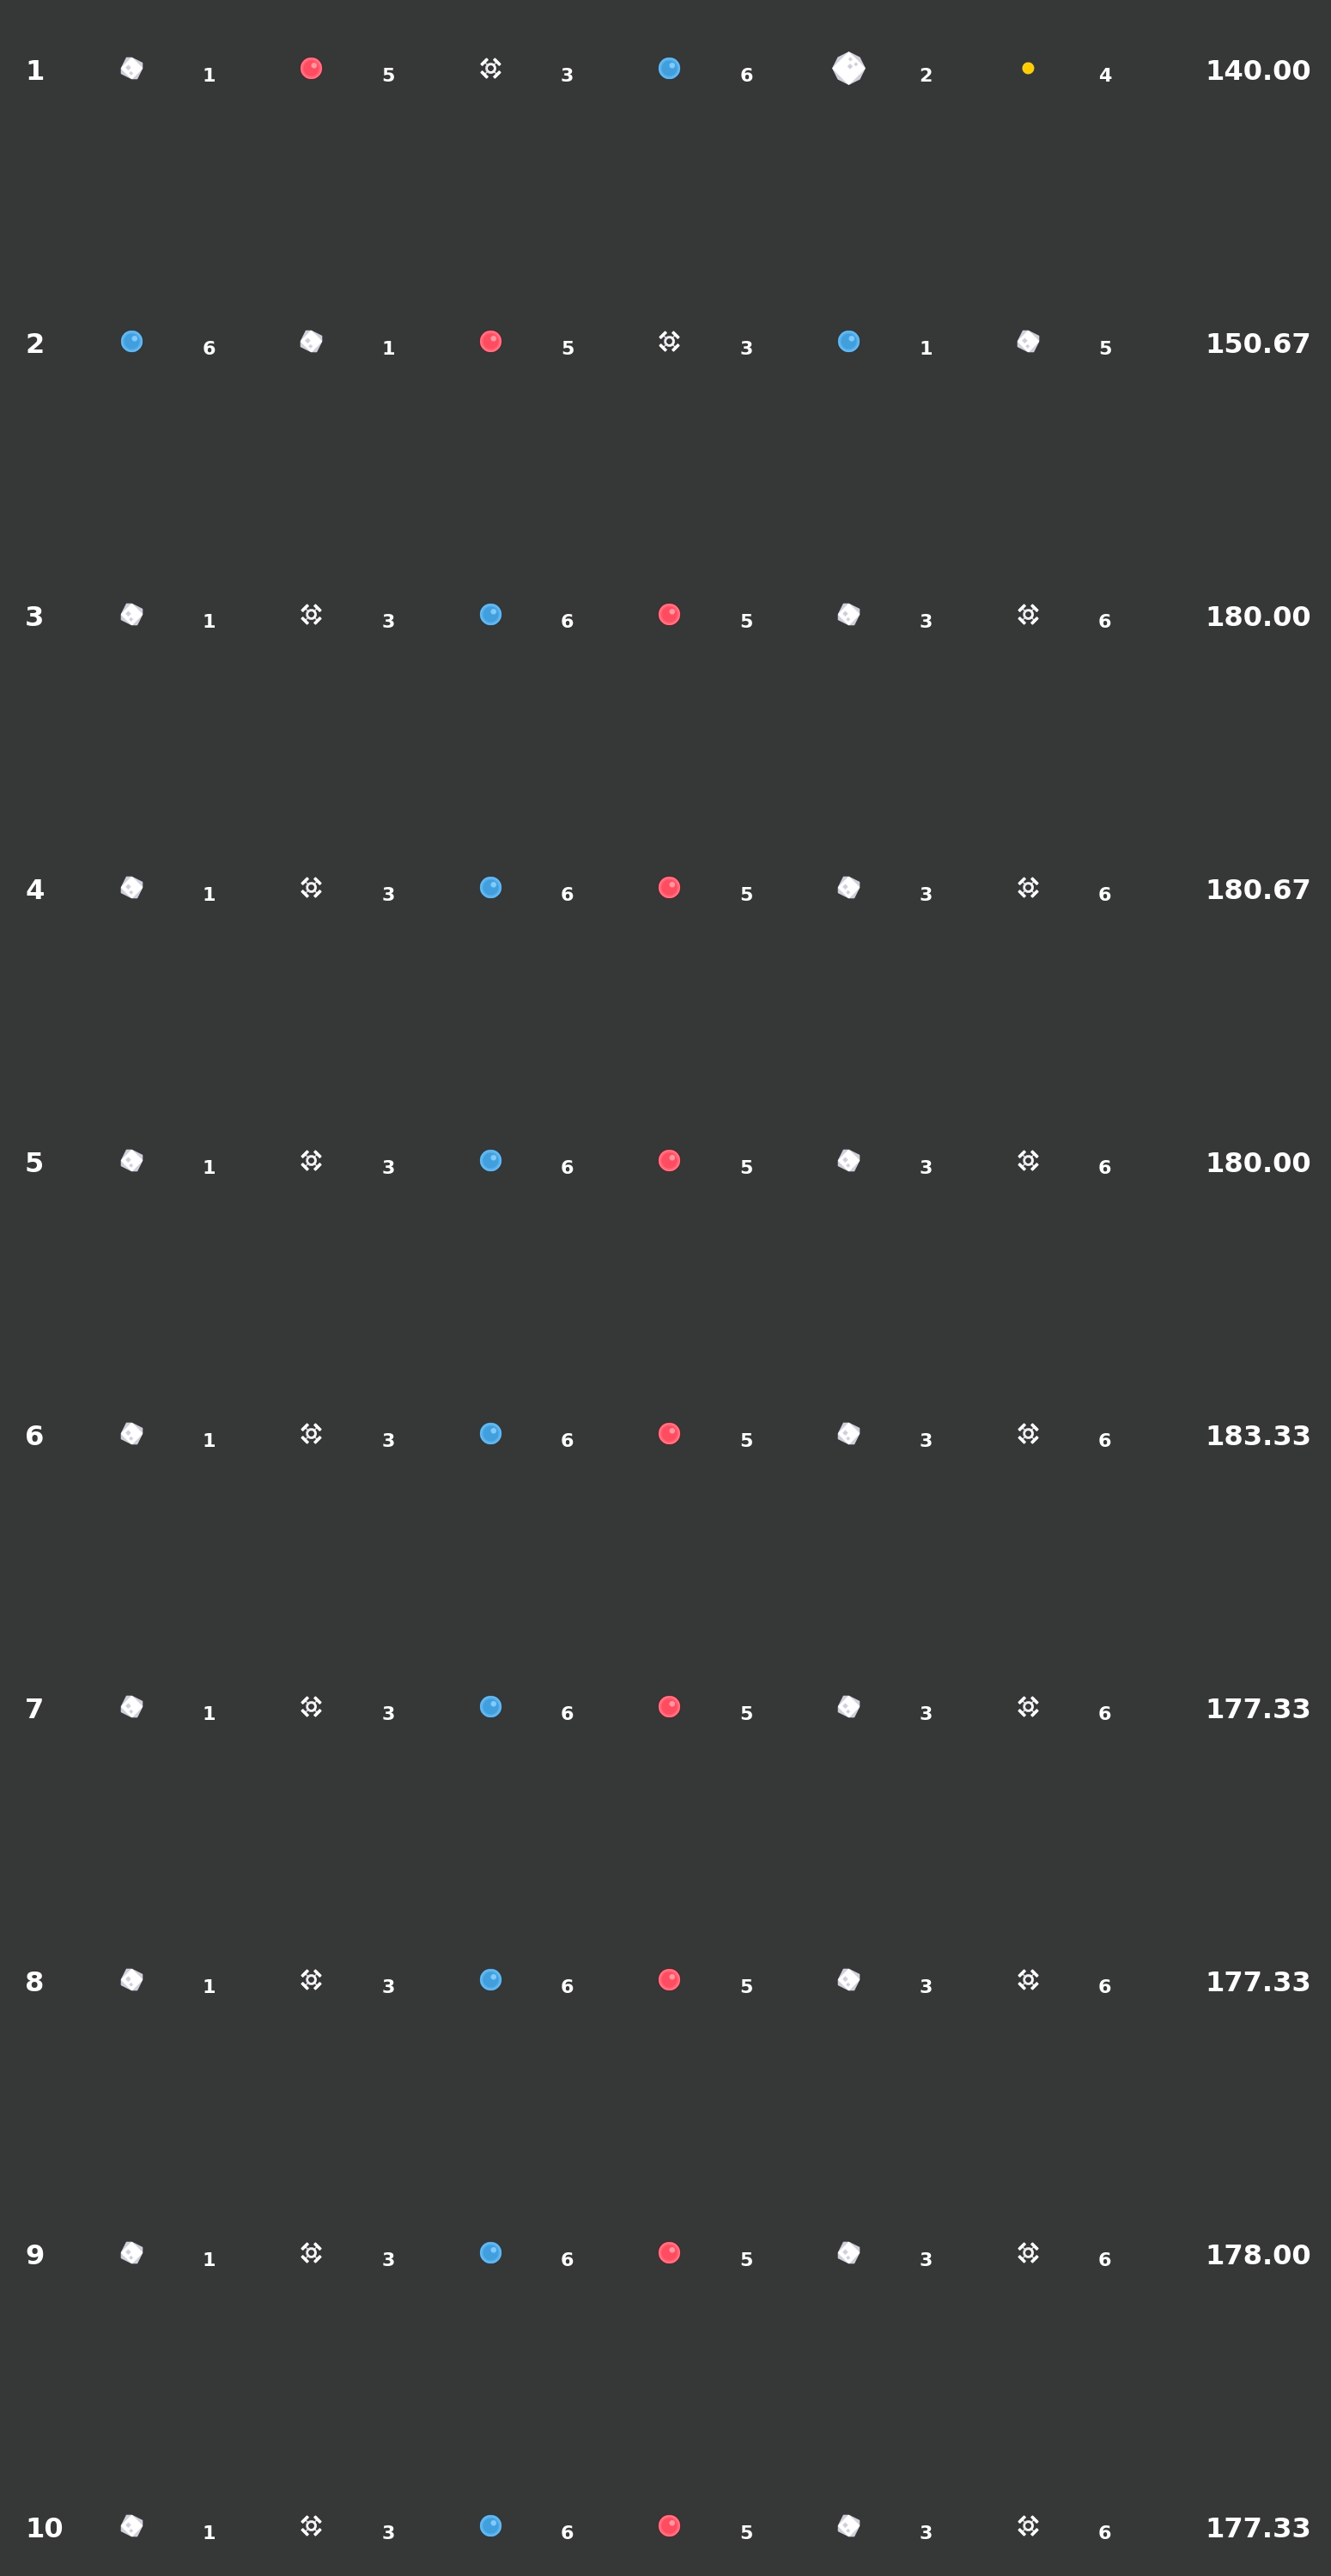
\includegraphics[width=0.7\textwidth]{figuras/ss/ss_redstill_ai_mode_2_1.png}
  \caption{Visualização da moda de cada onda com o fitness v3 contra Nave Parada, Disparo Vermelho.}
  \label{fig:ss-moda-rs-2-1}
\end{figure}

\begin{figure}[H]
  \centering
  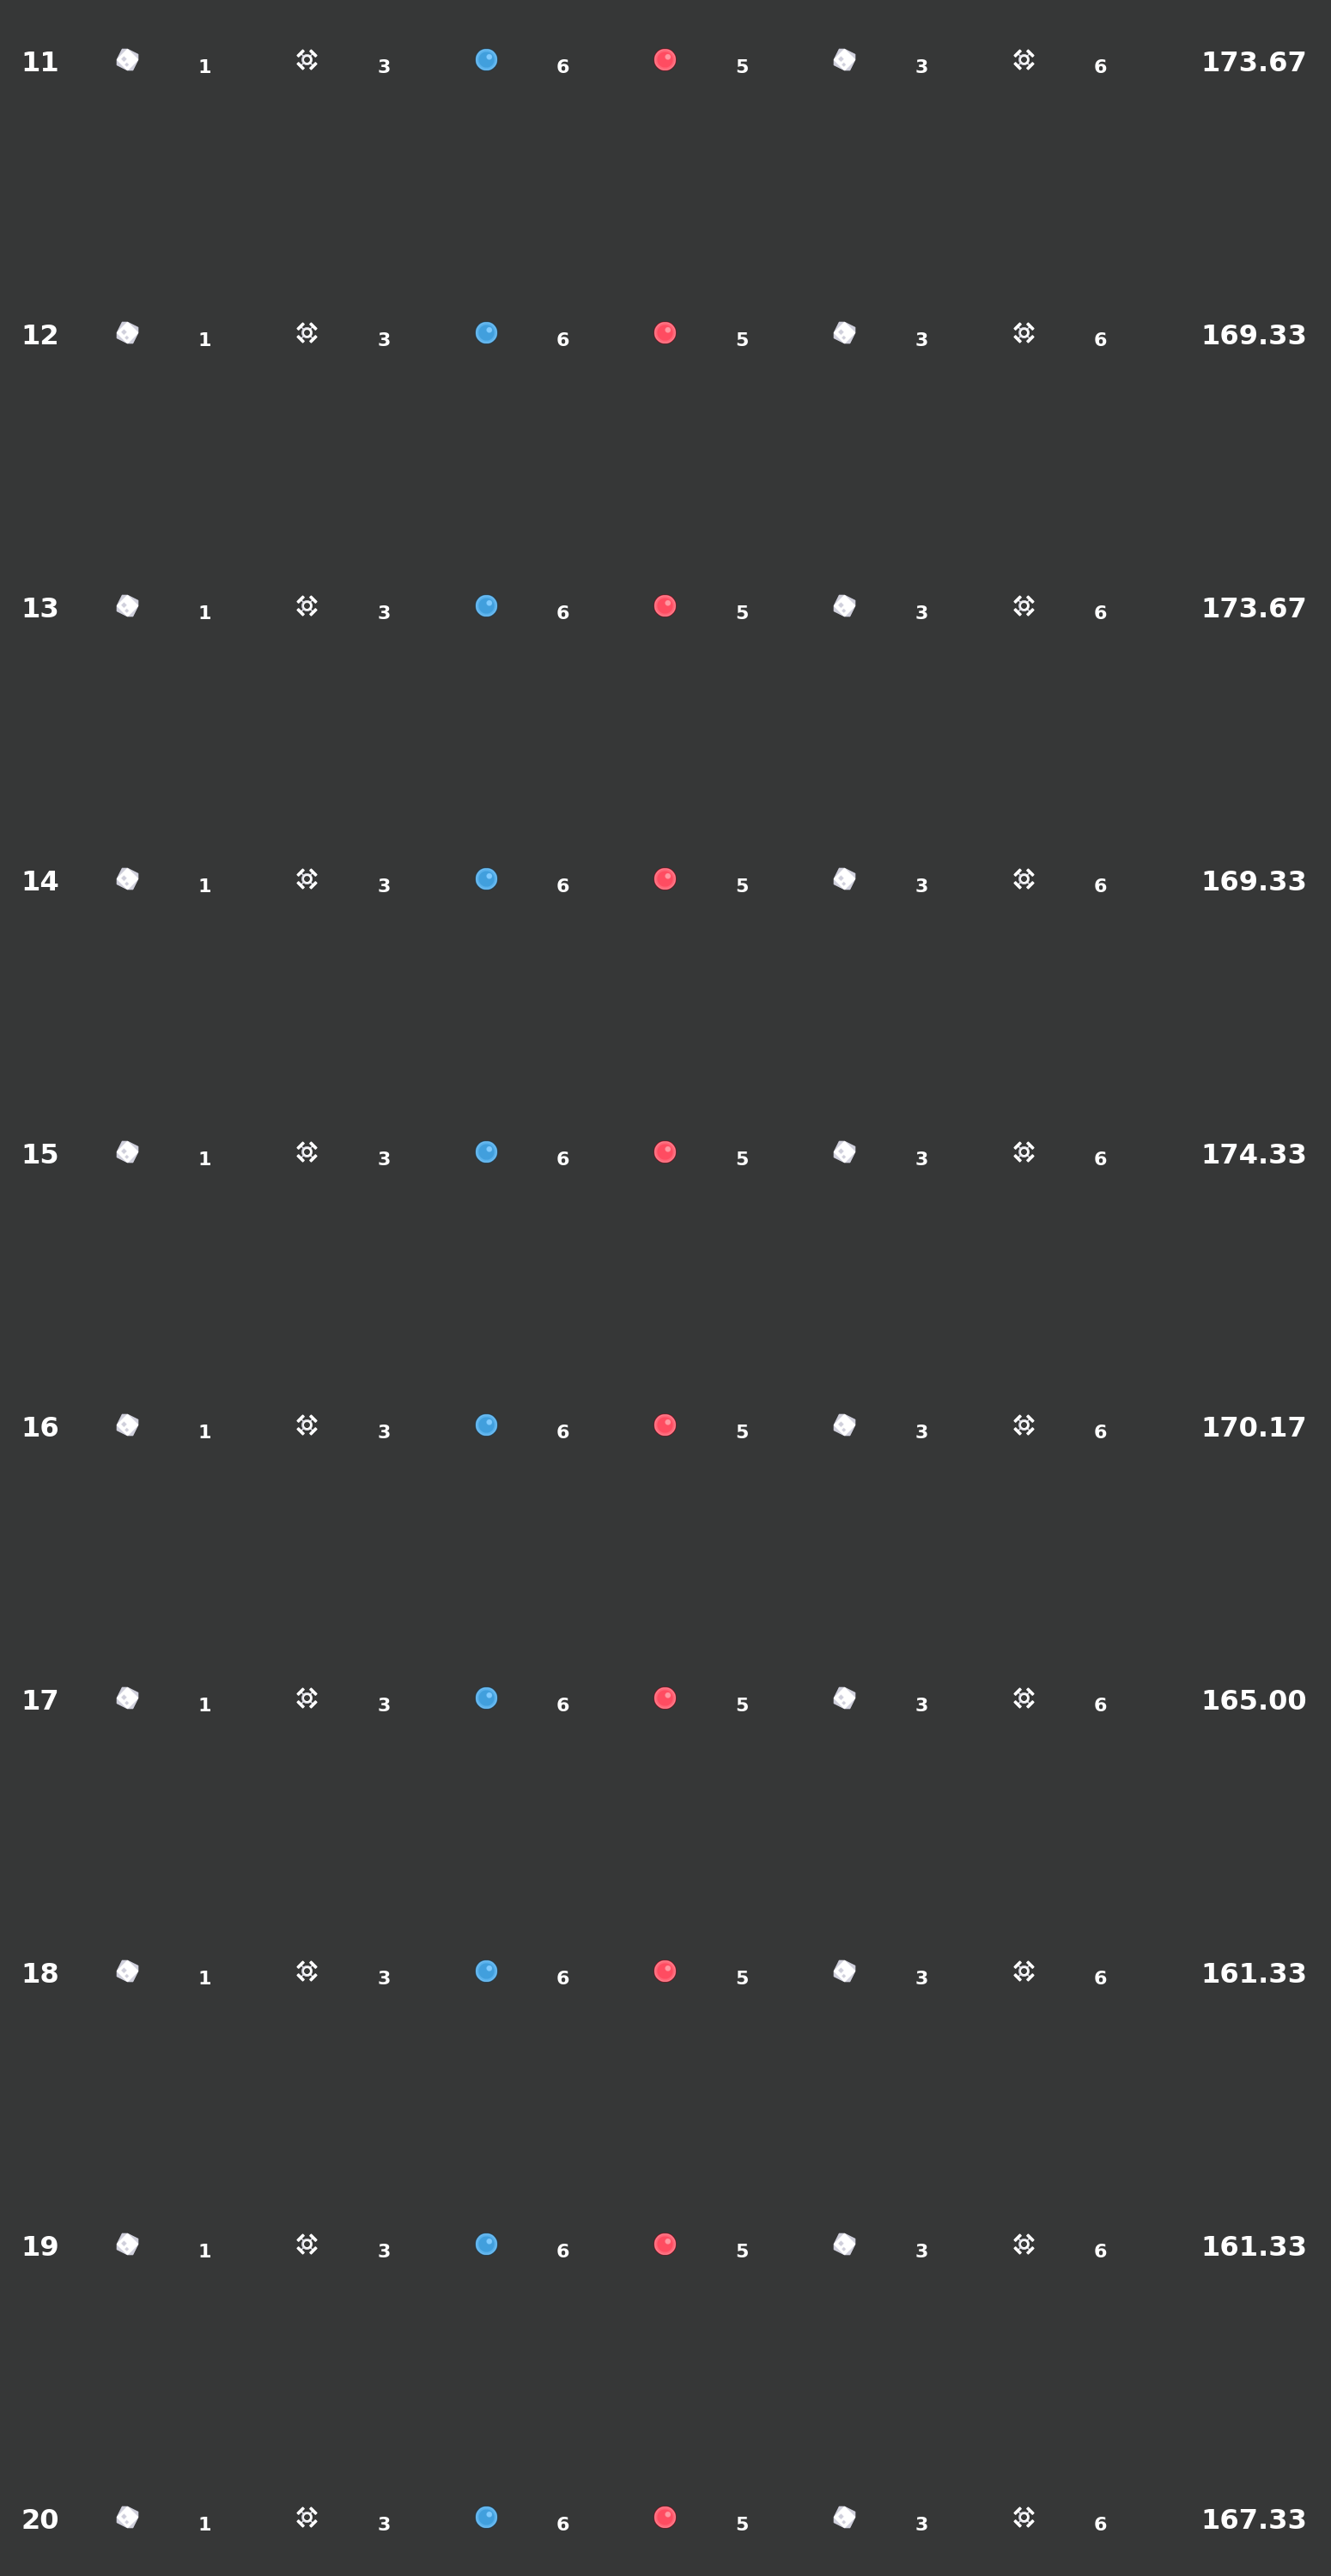
\includegraphics[width=0.7\textwidth]{figuras/ss/ss_redstill_ai_mode_2_2.png}
  \caption{Visualização da moda de cada onda com o fitness v3 contra Nave Parada, Disparo Vermelho.}
  \label{fig:ss-moda-rs-2-2}
\end{figure}

\begin{figure}[H]
  \centering
  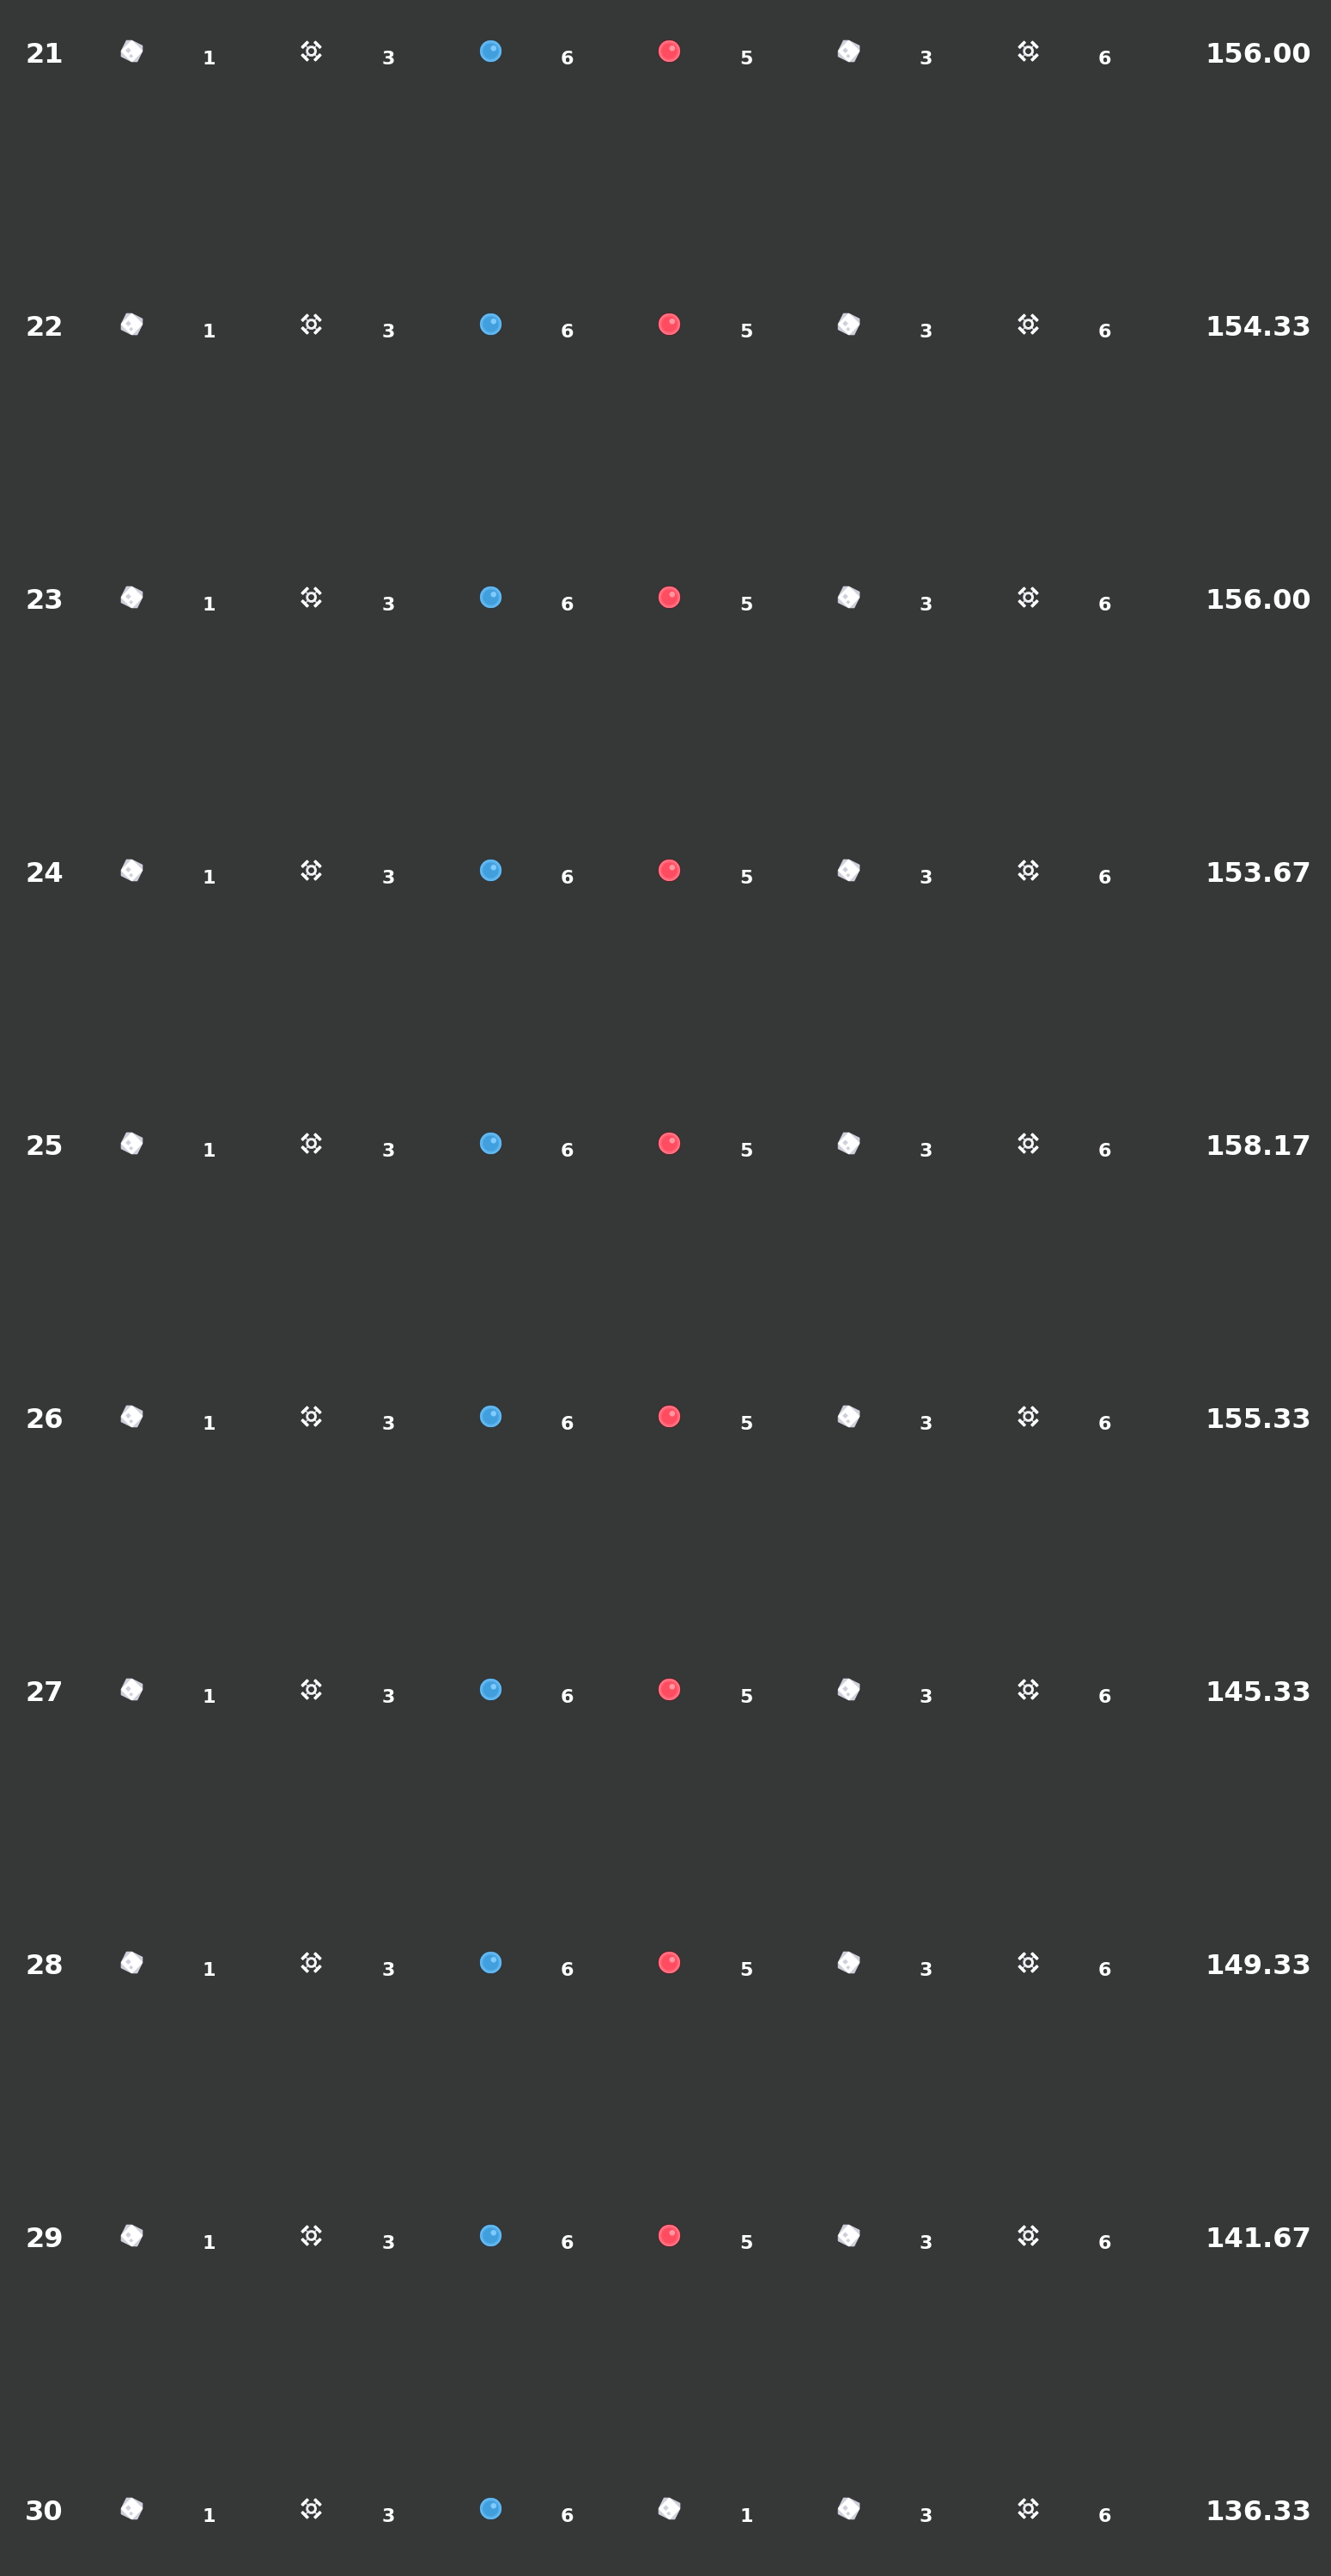
\includegraphics[width=0.7\textwidth]{figuras/ss/ss_redstill_ai_mode_2_3.png}
  \caption{Visualização da moda de cada onda com o fitness v3 contra Nave Parada, Disparo Vermelho.}
  \label{fig:ss-moda-rs-2-3}
\end{figure}

%% ------------------------------------------------------------------------- %%
\section{Nave Movendo com Disparo Vermelho}
\label{sec:apend-moda-ss-rm-v3}

\begin{figure}[H]
  \centering
  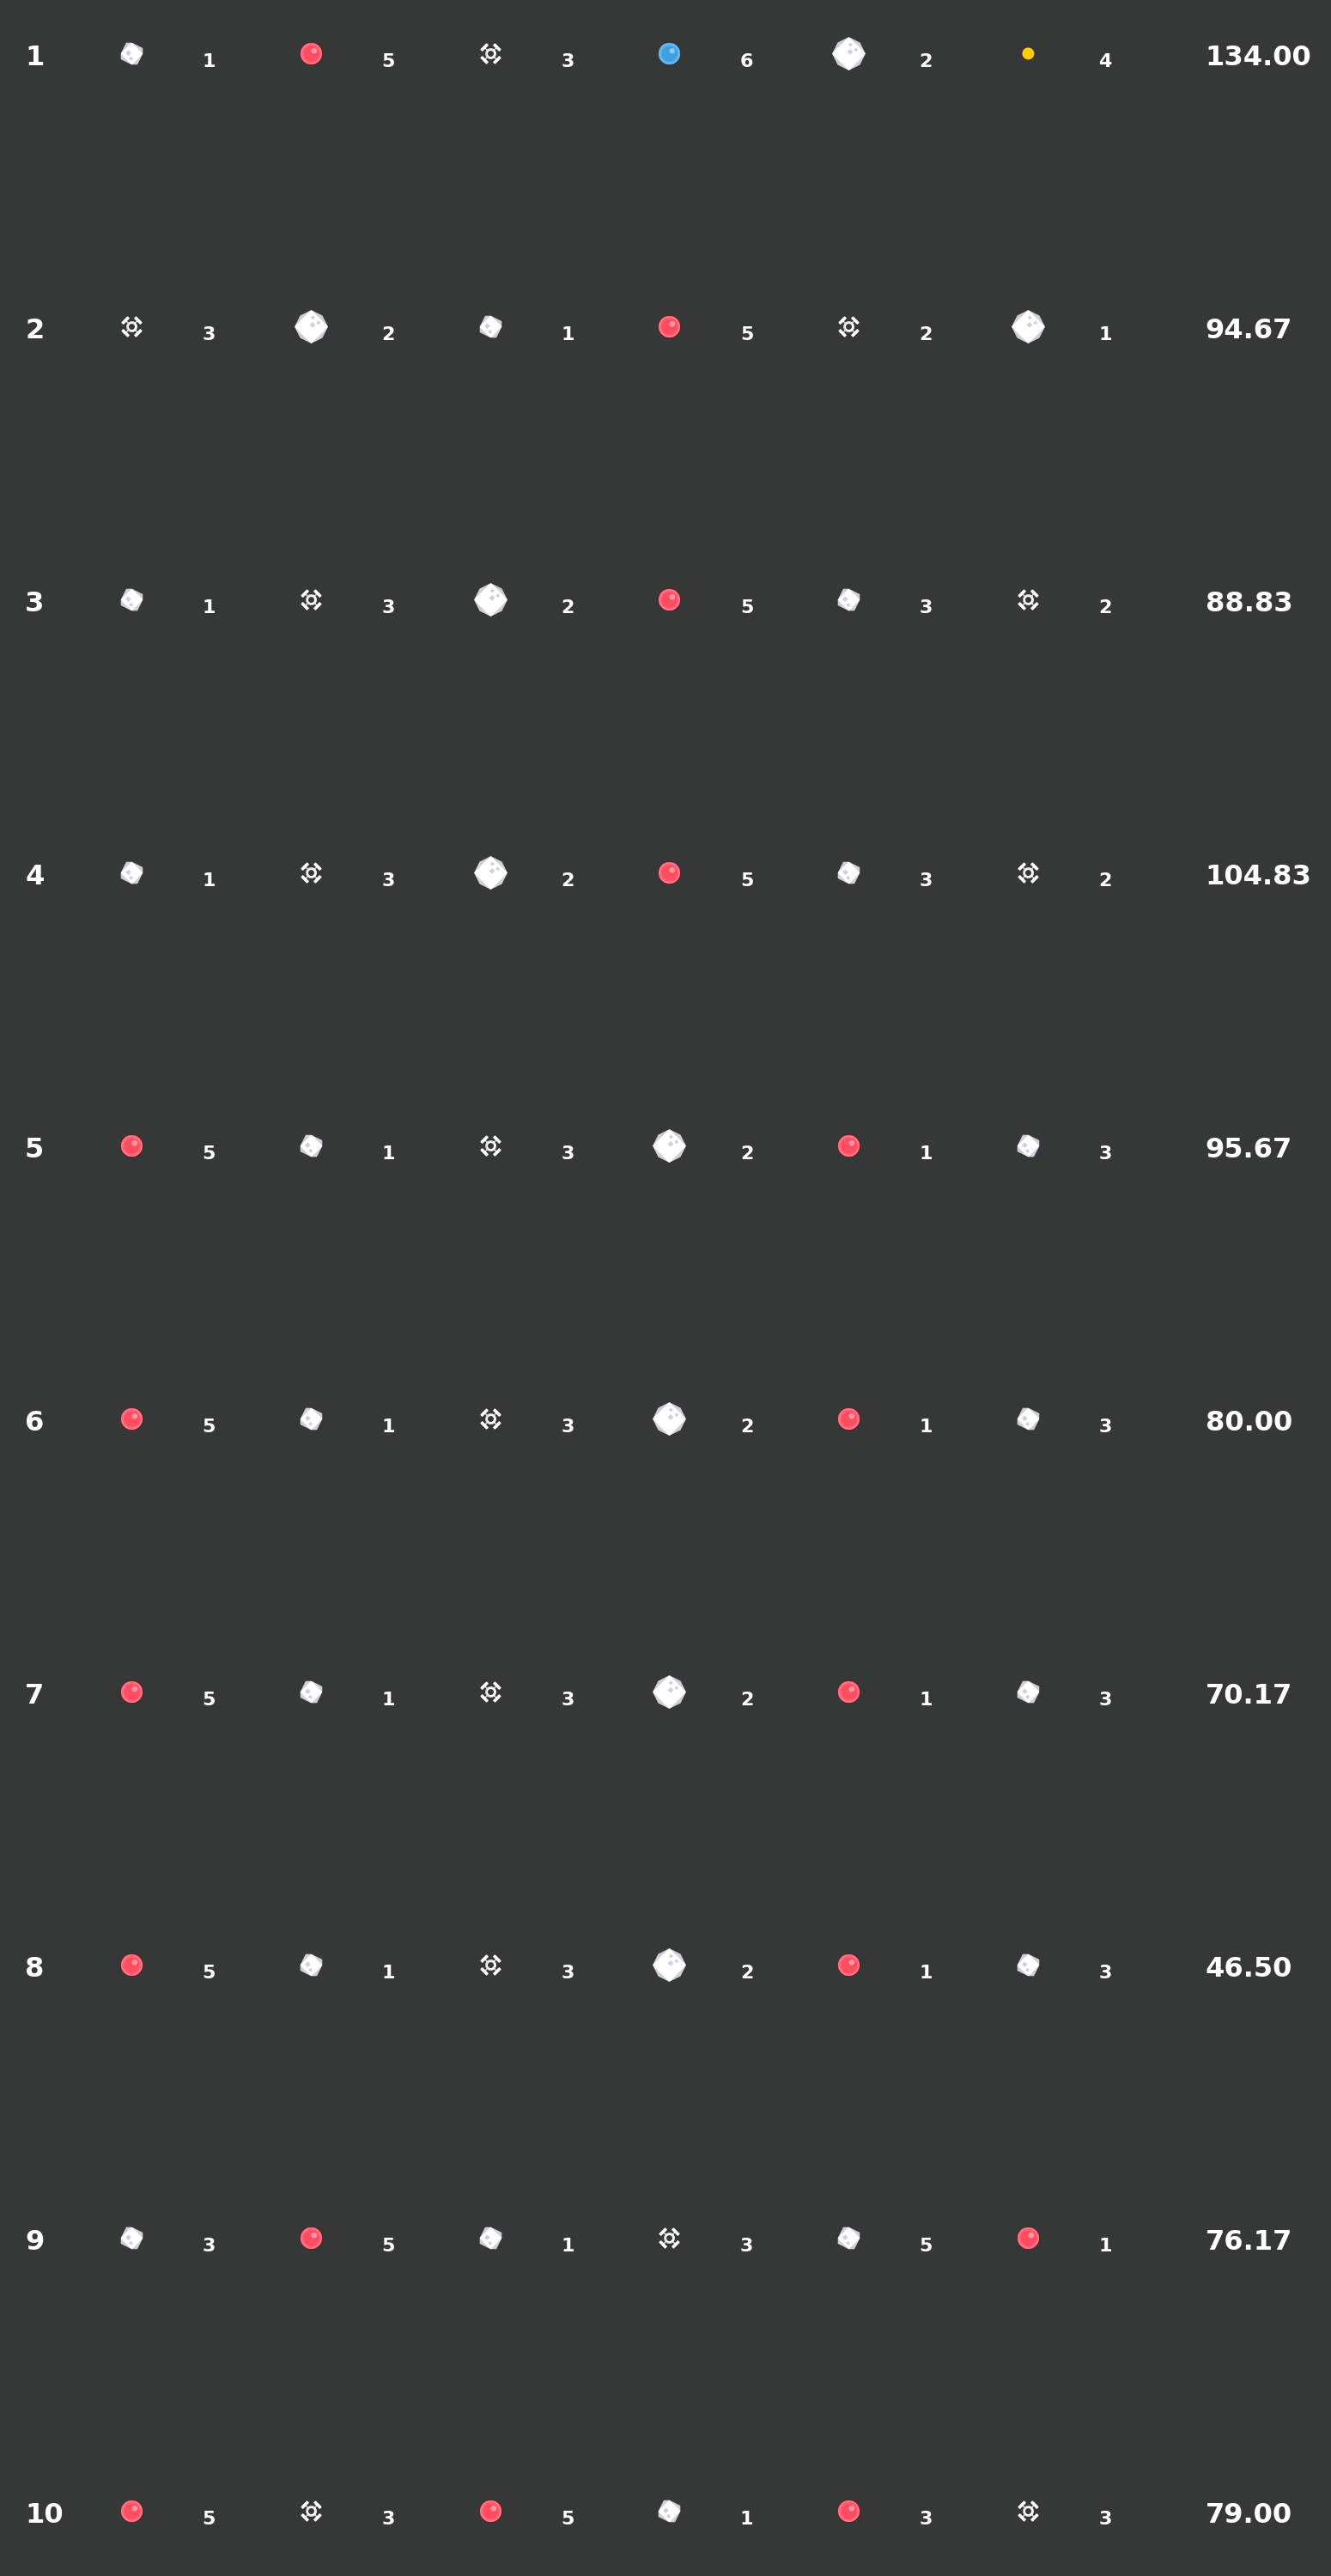
\includegraphics[width=0.7\textwidth]{figuras/ss/ss_redmove_ai_mode_2_1.png}
  \caption{Visualização da moda de cada onda com o fitness v3 contra Nave Movendo, Disparo Vermelho.}
  \label{fig:ss-moda-rm-2-1}
\end{figure}

\begin{figure}[H]
  \centering
  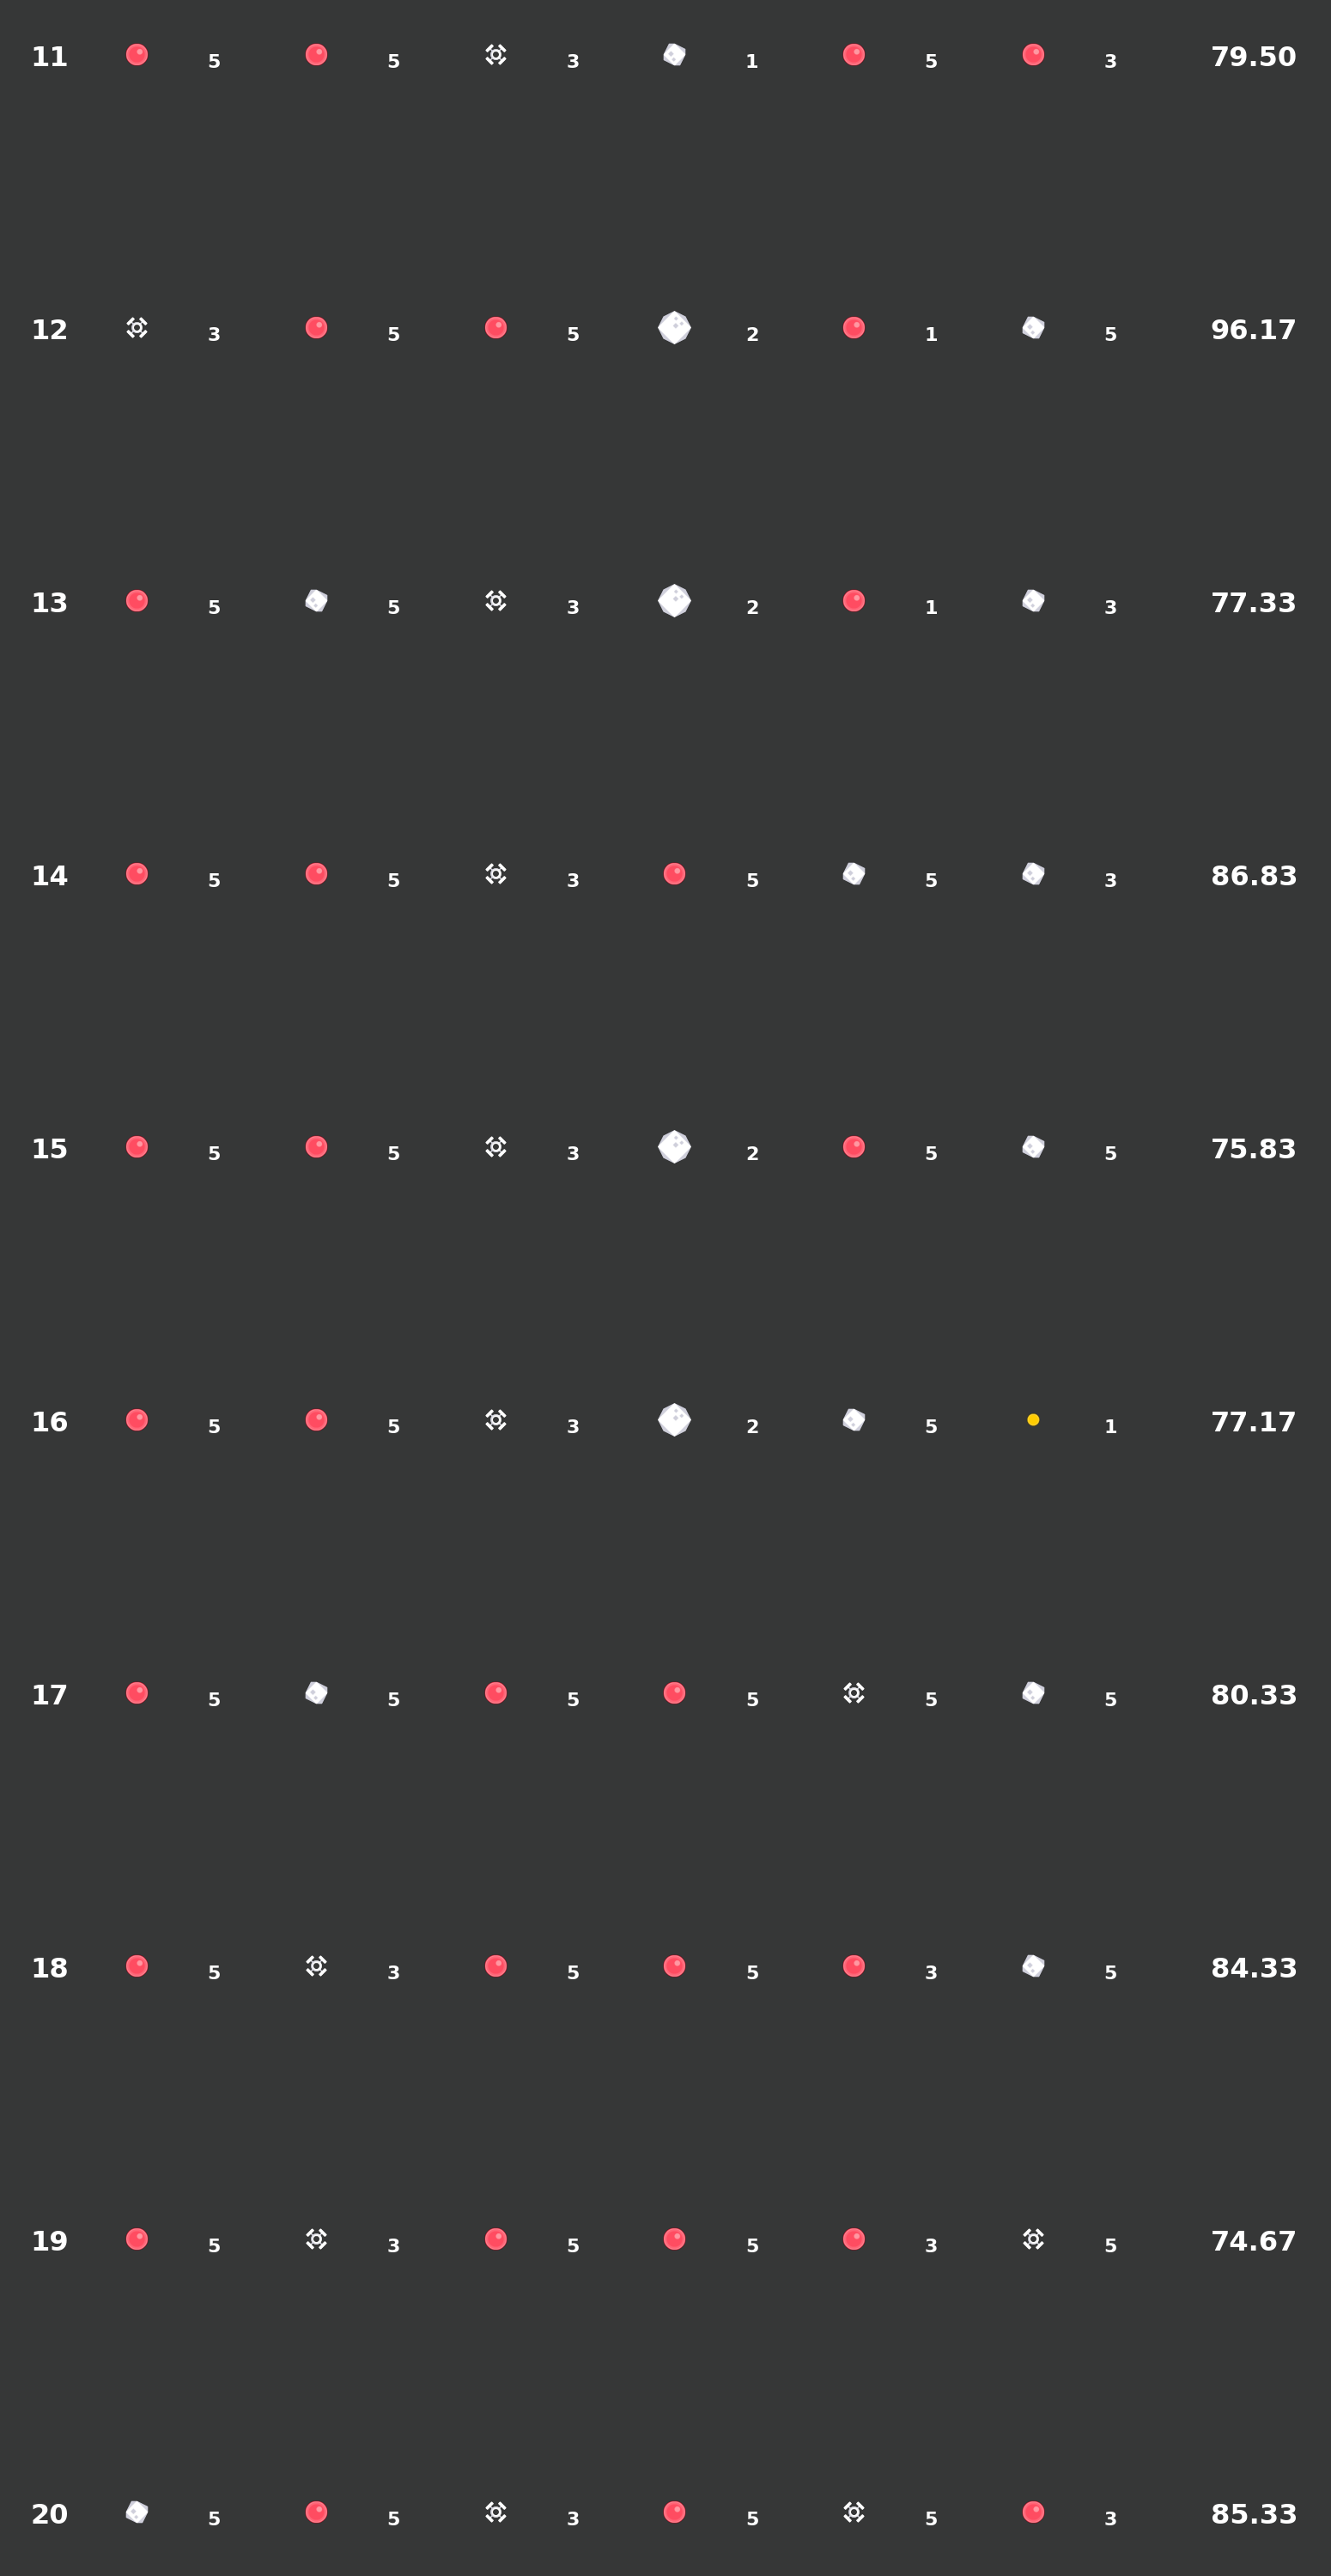
\includegraphics[width=0.7\textwidth]{figuras/ss/ss_redmove_ai_mode_2_2.png}
  \caption{Visualização da moda de cada onda com o fitness v3 contra Nave Movendo, Disparo Vermelho.}
  \label{fig:ss-moda-rm-2-2}
\end{figure}

\begin{figure}[H]
  \centering
  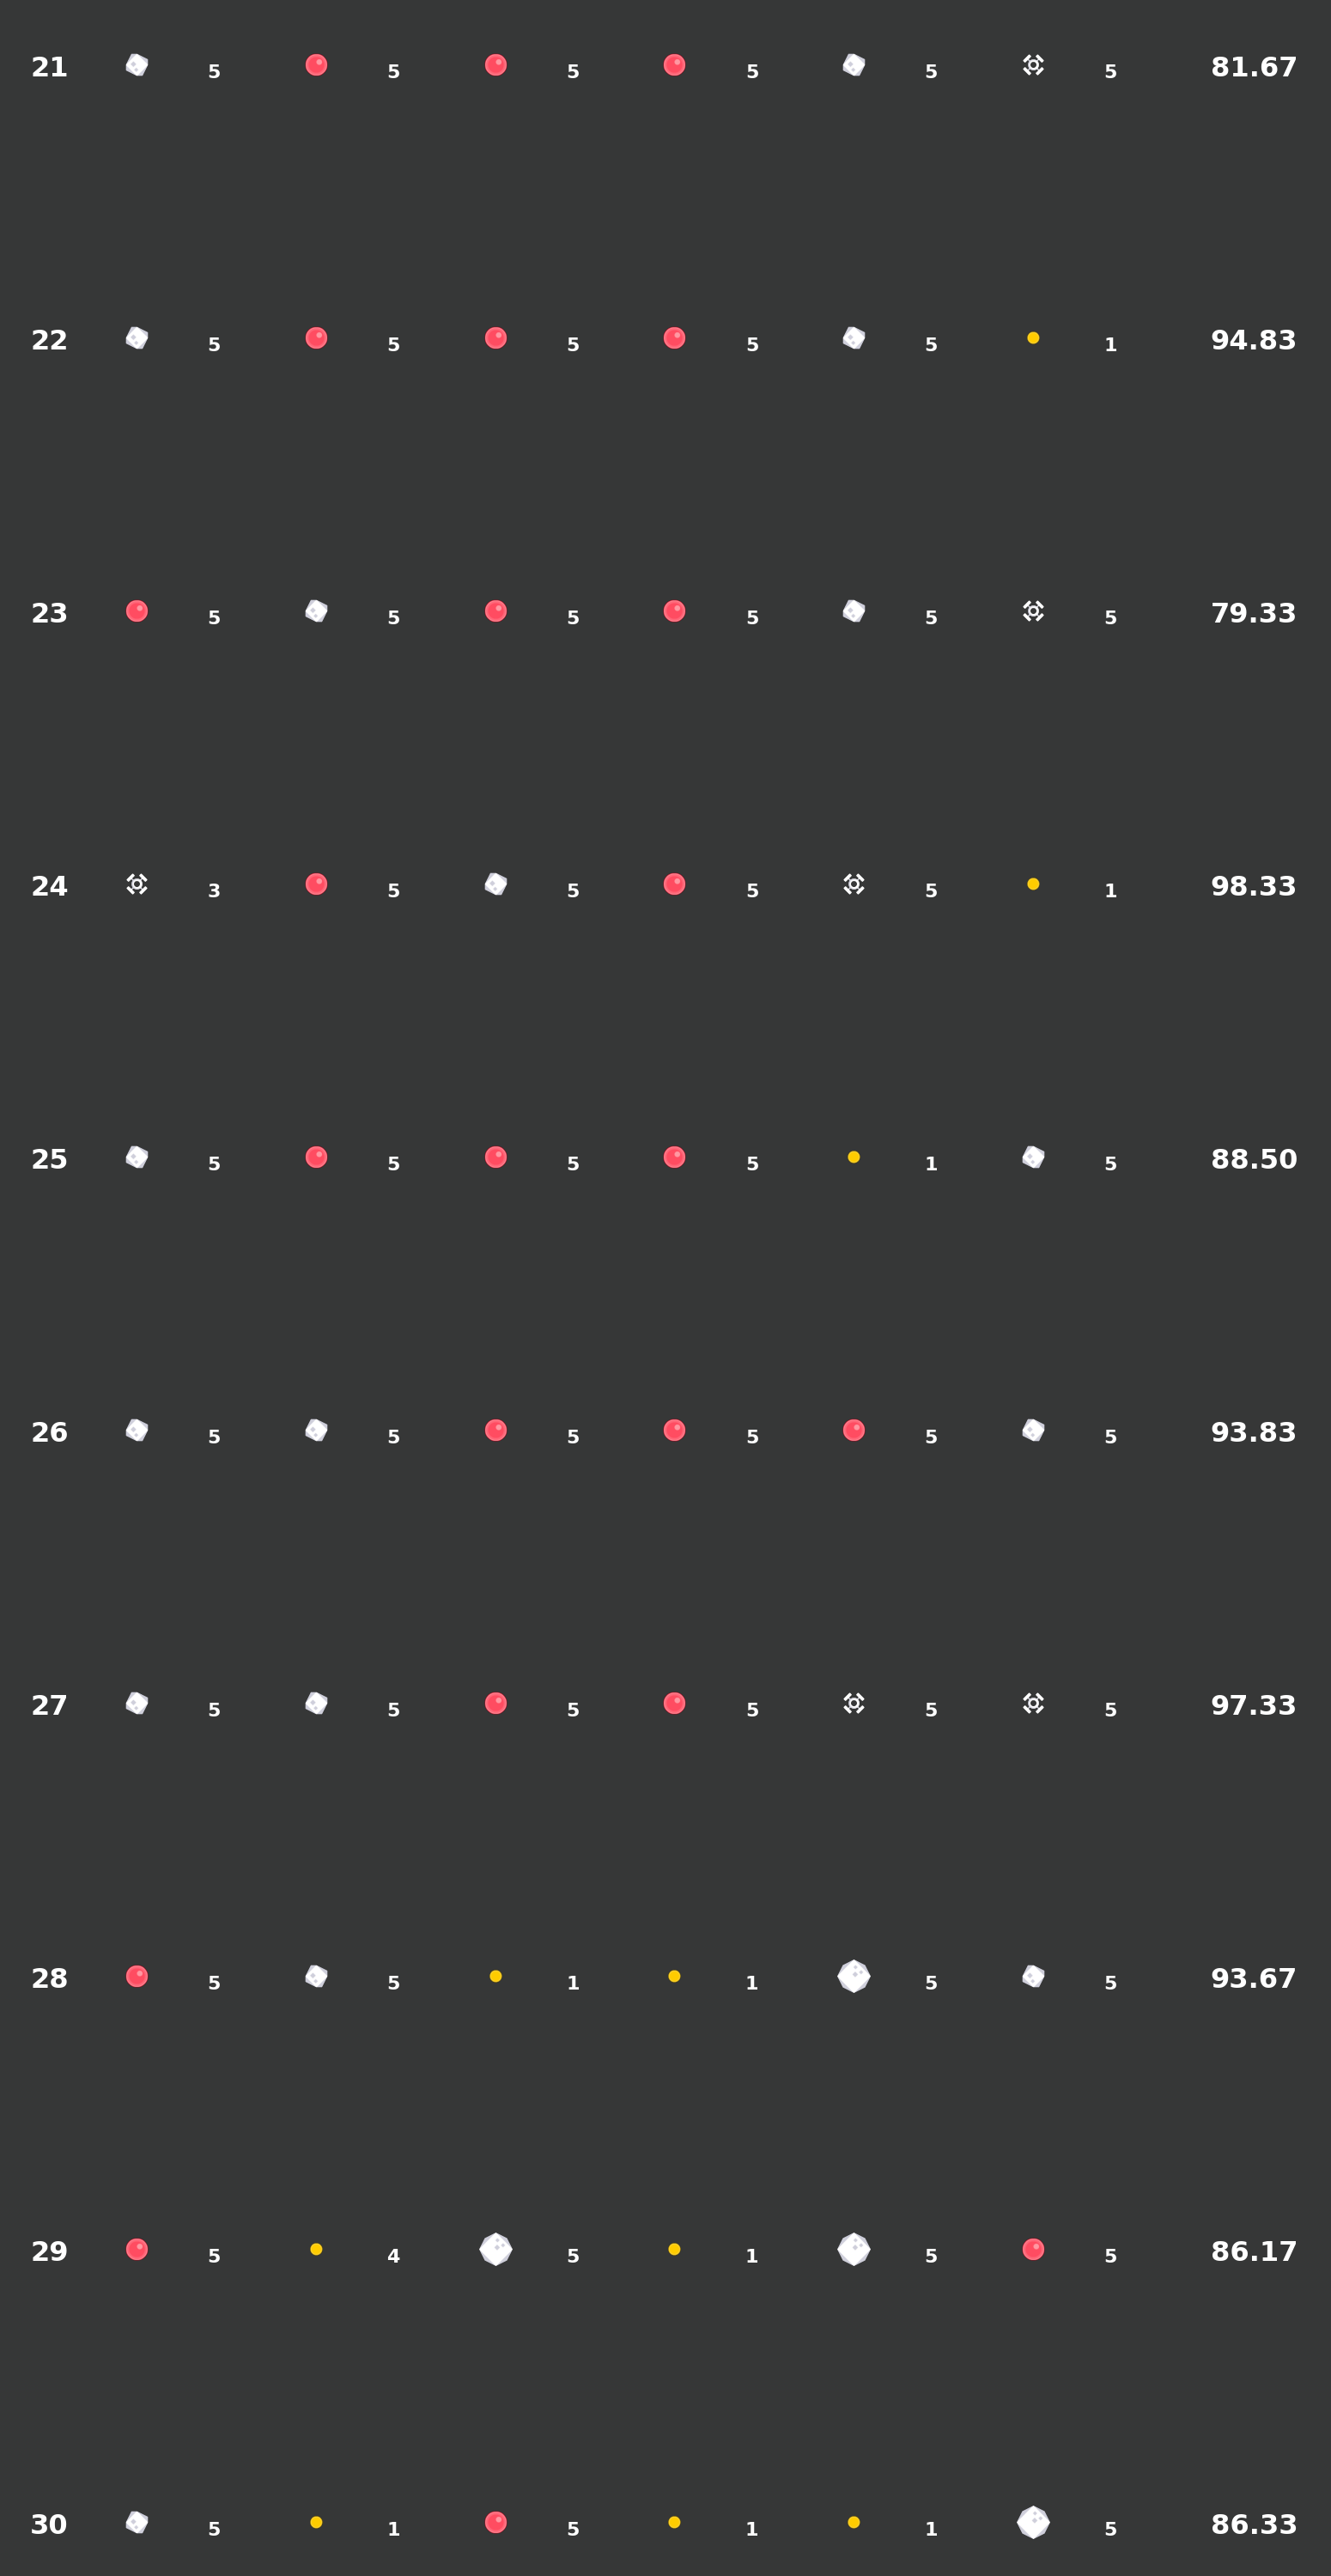
\includegraphics[width=0.7\textwidth]{figuras/ss/ss_redmove_ai_mode_2_3.png}
  \caption{Visualização da moda de cada onda com o fitness v3 contra Nave Movendo, Disparo Vermelho.}
  \label{fig:ss-moda-rm-2-3}
\end{figure}